\documentclass{../../text-style}

\texttitle{Системы контроля версий}

\begin{document}

\maketitle
\thispagestyle{empty}

\section{Введение}

Начнём с назначения систем контроля версий. Есть распространённое заблуждение, что они нужны в основном для командной работы, так что использовать их в одиночных проектах (например, НИР/курсовых/дипломах). На самом деле, основное назначение систем контроля версий --- хранить историю разработки, чтобы в любой момент иметь возможность вернуться к любому состоянию системы в прошлом. Систему контроля версий можно понимать как некую машину времени, которую можно использовать, если вы что-то напрограммировали, всё перестало работать и вы не помните, что меняли. Или обнаружился баг на релизной версси, который на текущем варианте исходников не воспроизводится. Или есть баг, который вы никак не можете локализовать, и вам надо понять, начиная с какой версии он начал воспроизводиться и какие именно в этой версии поменялись строки кода. Так что даже если вы работаете в одиночку, системы контроля версий необходимы --- как ремни безопасности. Без них есть большой риск за один раз потерять всю свою работу, а поскольку программные проекты обычно длятся месяцы, а то и годы, ни один нормальный человек без системы контроля версий ничего больше сотни строк кода писать не будет.

Кроме того, все нормальные системы контроля версий поддерживают ветки. Ветки --- это по сути альтернативна история изменений кода, когда на базе одной и той же версии можно попробовать сделать так, а можно --- этак. Это позволяет безопасно (ведь всегда можно вернуться к исходной версии) и удобно (ведь переключаться между ветками легко) пробовать разные варианты решения задачи, не мешать друг другу при командной разработке, иметь отдельные ветки для разных релизов, где потом спокойно делать хотфиксы и не бояться ничего сломать, и т.д. Плюс к тому, ветки можно объединять --- если ваш эксперимент удался, его можно легко и часто полностью автоматически влить в основной вариант кода. То есть система контроля версий --- это не просто машина времени, но машина времени с несколькими альтернативными историями, которые могут разделяться и сливаться.

Ну и конечно, системы контроля версий необходимы для командной разработки. Причём в двух качествах --- как централизованное хранилище кода и как способ друг другу не мешать и легко распространять изменения. Как централизованное хранилище кода системы контроля версий особенно хороши вместе с облачными хостингами типа GitHub --- никто не мешает вам держать весь репозиторий у себя локально, но если у вас сломается жёсткий диск, то всё. Облачные сервисы, как правило, имеют очень продвинутую инфраструктуру для обеспечения надёжности. Ну и когда код проекта доступен из любой точки земного шара, это сильно помогает распределённым командам координироваться.

\subsection{Виды систем контроля версий}

Мудрые, но необразованные люди часто сами приходят к идее контроля версий на локальном компьютере или сетевой шаре: допрограммировали до какой-то работоспособной версии --- отложили в отдельную папку, как на рисунке:

\begin{center}
    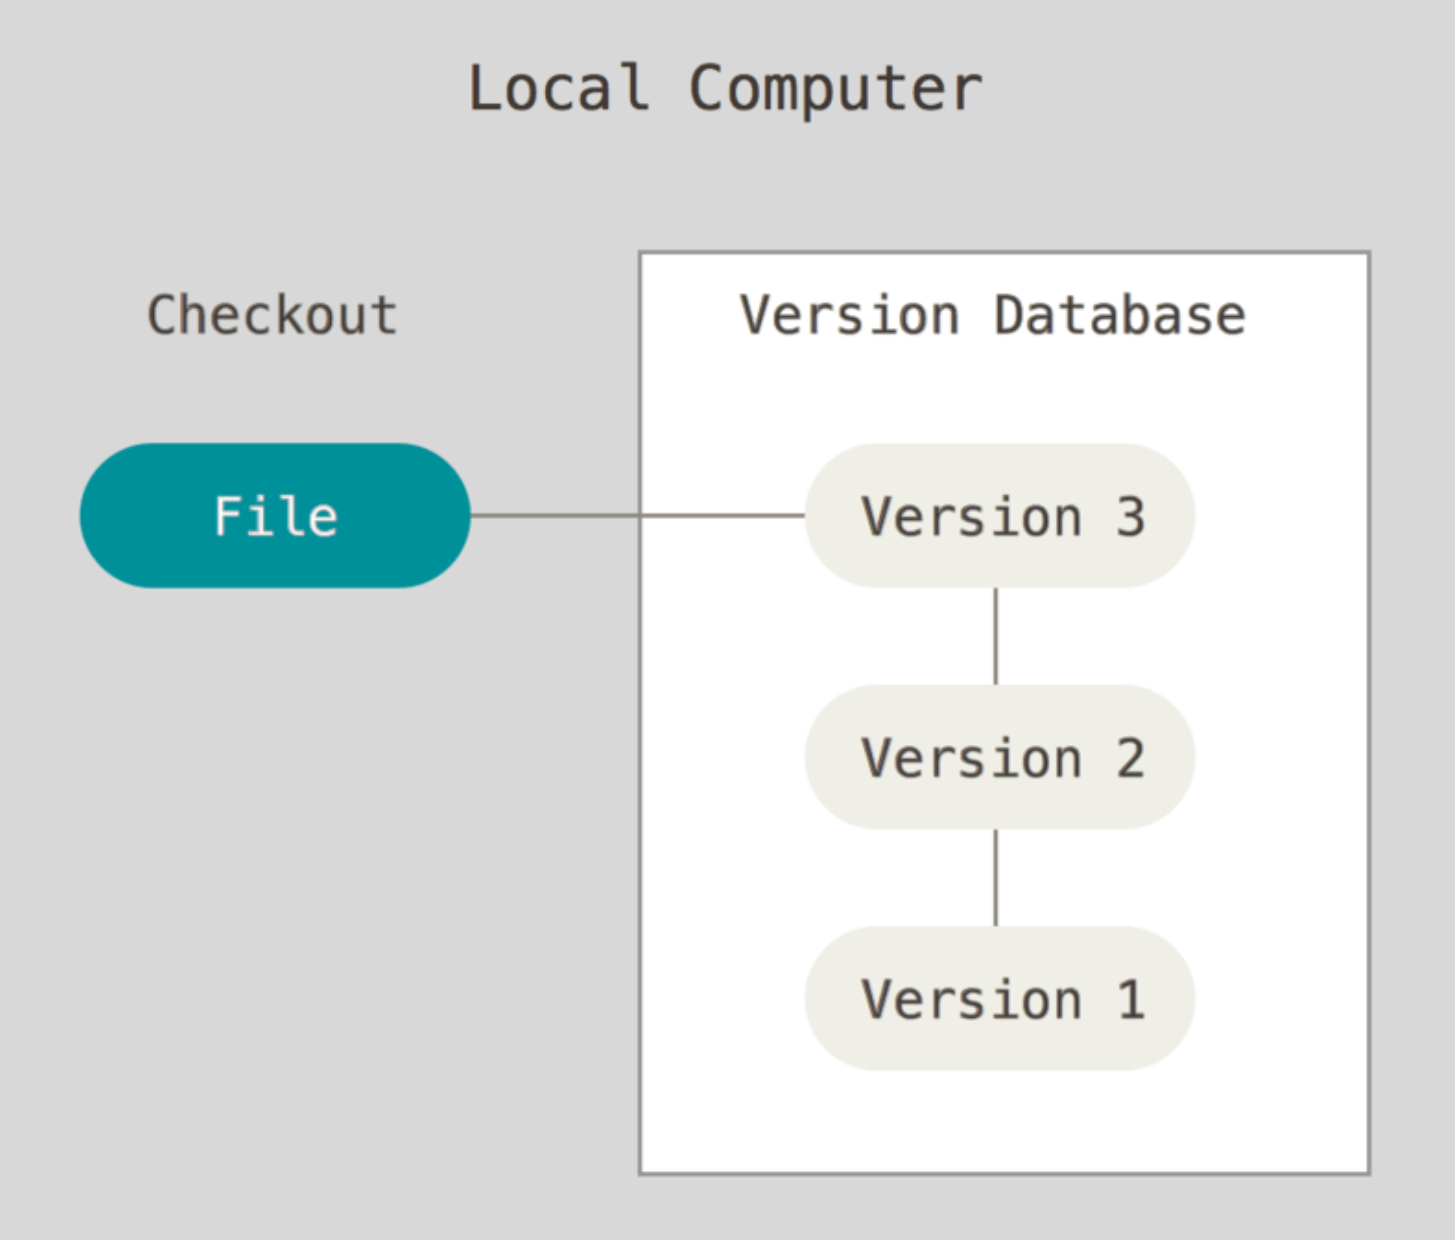
\includegraphics[width=0.5\textwidth]{localCopies.png}
    \attribution{https://git-scm.com/book/ru}
\end{center}

Автор сам так делал на заре своей профессиональной карьеры (справедливости ради, системы контроля версий того времени --- начала 2000-х --- были не очень удобны в использовании, так что в те времена это был вполне вариант).

Однако сейчас так делать нельзя --- системы контроля версий нынче очень хороши, полностью автоматизируют создание резервных копий и делают ещё много чего хорошего, часть из чего перечислена выше. 

Систем контроля версий бывает два вида --- централизованные и распределённые. Пример централизованной системы --- Subversion, очень популярная в 2000-х и иногда используемая до сих пор\footnote{На самом деле, если вы работаете в одиночку, вам не очень нужны ветки и всегда есть доступ в интернет, Subversion может оказаться вдвое удобнее распределённых систем, просто потому что на выкладывание очередной версии требует одну команду, а не две. Я не знаю, зачем выкладываю эти конспекты в Git, а не в Subversion...}. Там все версии хранятся в одном репозитории, а каждый клиент может лишь получить текущую рабочую копию. После внесения изменений пользователь должен выложить их на сервер, иначе они не зафиксируются. Это хорошо тем, что есть единственный центральный источник исходников для всего проекта, плохо тем, что требуется сетевое подключение даже для таких частых операций, как коммит. Концептуально централизованные системы устроены так:

\begin{center}
    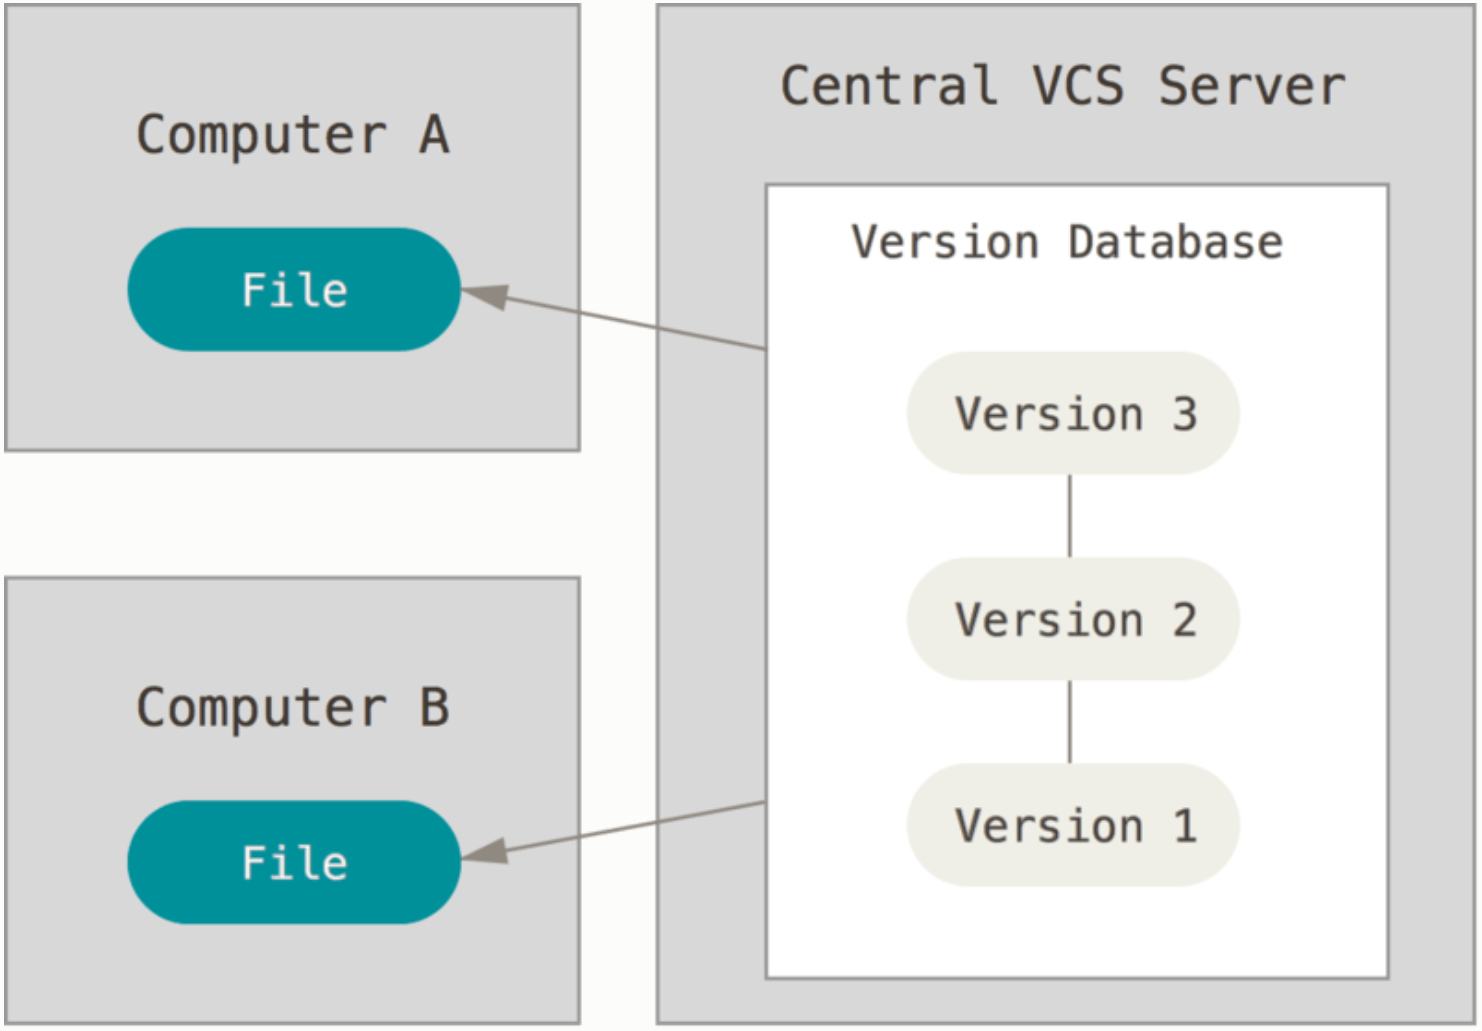
\includegraphics[width=0.5\textwidth]{centralizedVcs.png}
    \attribution{https://git-scm.com/book/ru}
\end{center}

Распределённые системы предполагают, что у каждого разработчика своя собственная копия репозитория и репозитории могут обмениваться изменениями, кто угодно с кем угодно. При этом обычно чисто административно назначают центральный репозиторий, через который идёт обмен, и который хранит <<основной>> код разрабатываемой системы, но ничто не мешает так не делать и синхронизироваться по сколь угодно сложной топологии. Преимущества такой системы --- большая <<свобода>> в разработке, каждый может сделать себе точную копию проекта и разрабатывать его сам (со своей командой); операции типа коммитов могут выполняться локально (раз у каждого разработчика полный репозиторий), в любой момент времени доступна вся история проекта, без необходимости подключаться к серверу. Недостатки --- возможно, больший бардак (некоторые проекты имеют сотни форков, и никто не может сказать, какой из них самый актуальный), необходимость каждому разработчику локально хранить всю историю (так что если кто-то случайно выложил четырёхгиговый фильм и тут же его удалил, его всё равно все скачают, потому что в истории он останется). Популярные распределённые системы контроля версий --- Git и Mercurial.

Концептуально схема работы распределённых систем выглядит так:

\begin{center}
    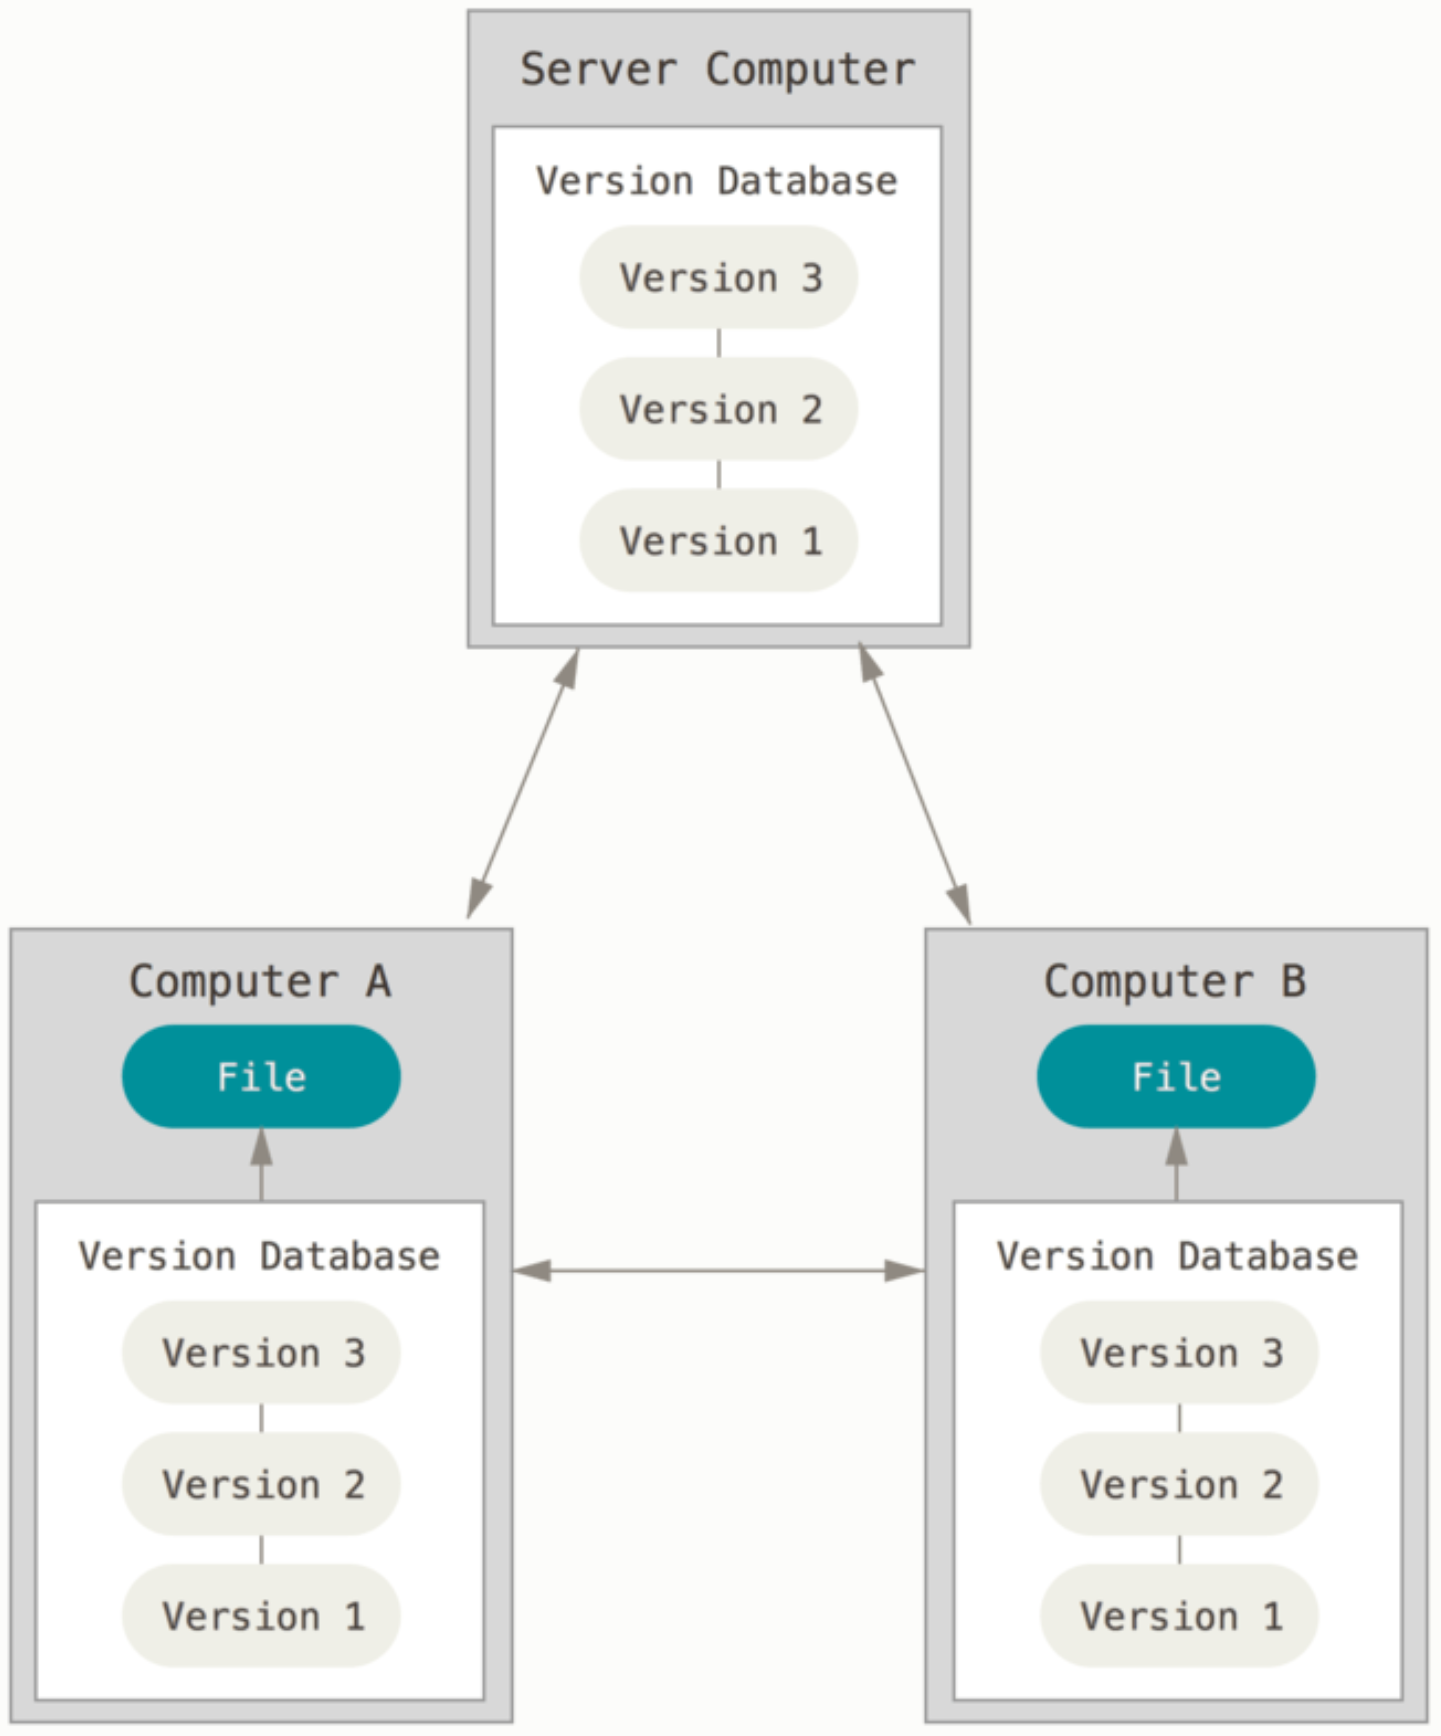
\includegraphics[width=0.55\textwidth]{distributedVcs.png}
    \attribution{https://git-scm.com/book/ru}
\end{center}

\subsection{Версионирование, дельты}

Любая современная система контроля версий работает не с файлами, а с изменениями. Базовой единицей версионирования является коммит --- набор изменений. Коммит состоит из дельт, каждая из которых хранит информацию об изменении в каждом файле версионируемых исходников. Вот так, например, дельта выглядит на GitHub:

\begin{center}
    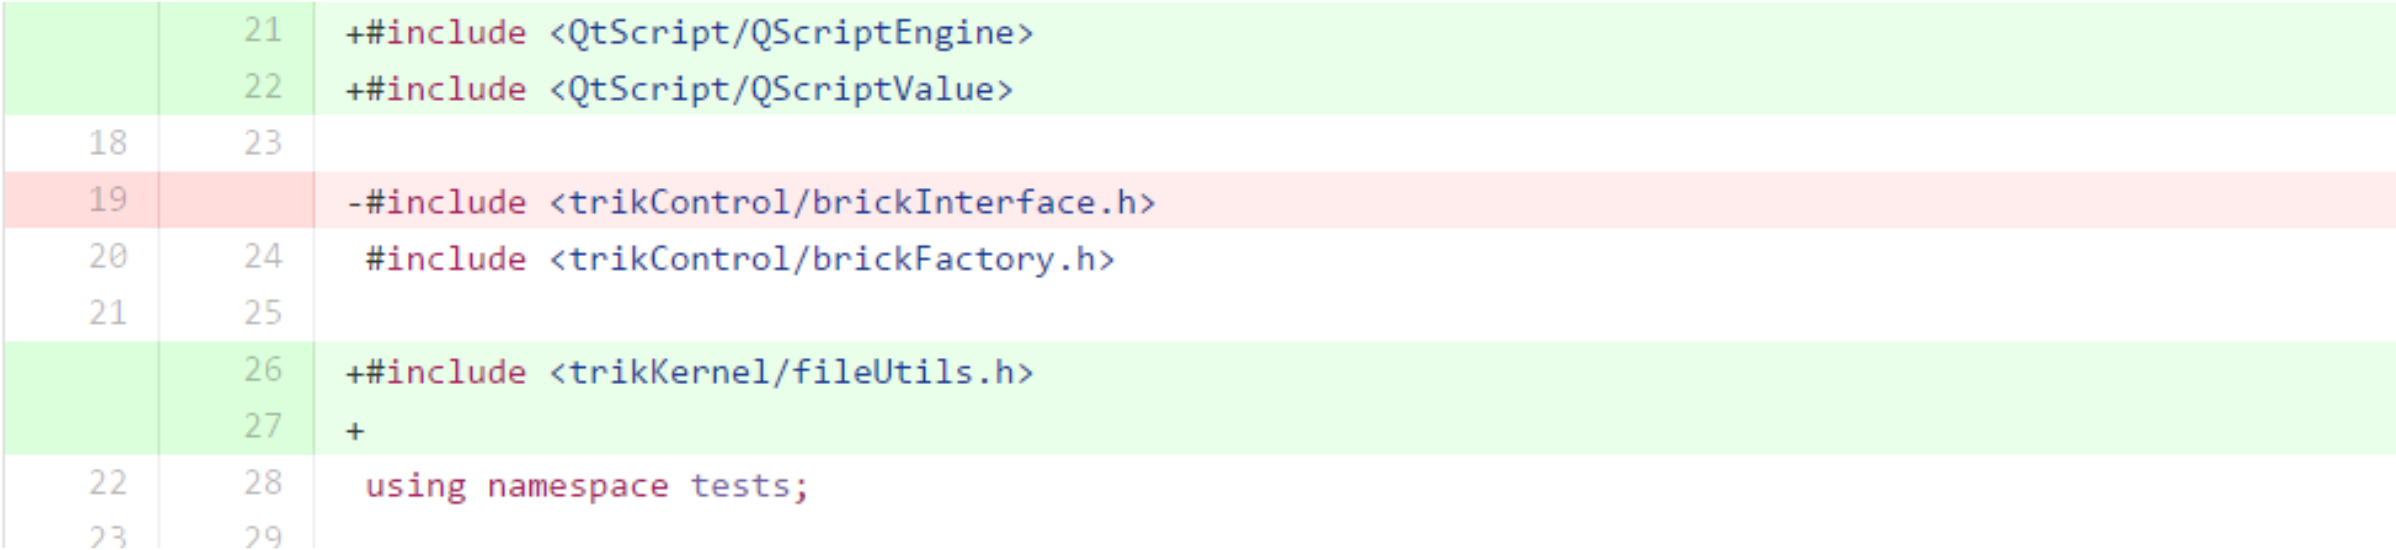
\includegraphics[width=0.9\textwidth]{delta.png}
\end{center}

Тут зелёным выделены новые строки, красным --- удалённые относительно предыдущей версии. Если файл в данной версии не менялся, то и в дельту он не попадёт, что позволяет эффективно хранить изменения в системе контроля версий --- как правило, каждый коммит затрагивает только единицы файлов, и остальные сотни тысяч файлов проекта остаются как есть. Также часто используются алгоритмы дельта-компрессии --- когда для каждого коммита хранятся реально только дельты, и текущая версия файла строится по исходной версии последовательным применением коммитов, которые затрагивали этот файл. Однако не всегда --- например, Git в большинстве случаев хранит изменённые файлы целиком.

Для того, чтобы сформировать коммит, система контроля версий обычно хранит рядом с исходниками версию на момент последнего коммита (например, Git, будучи распределённой системой контроля версий, хранит весь репозиторий целиком в папке .git, и <<как было>> --- записано в файле <<index>>, лежащем в этой папке). Редактируют программисты <<рабочую копию>> --- обычные исходники, под управлением системы контроля версий, которые при коммите сличаются с <<как было>>. Обратите внимание, работа ведётся в папке с репозиторием прямо, пользователю никакие файлы никуда вручную копировать не нужно.

\section{Git}

Рассмотрим самую популярную на данный момент систему контроля версий --- Git. Git, скорее всего, так или иначе многим знаком, многие может даже пользовались, поэтому начнём с обсуждения некоторых мифов и недопониманий вокруг этой системы контроля версий.

\begin{enumerate}
    \item Git и GitHub --- разные вещи. Git --- это собственно система контроля версий, библиотека и консольная утилита, позволяющая ей удобно пользоваться. GitHub --- облачный хостинг репозиториев Git, которым владеет Microsoft\footnote{Не так давно его купила, кстати.} и который бесплатен для проектов с открытым исходным кодом, но вообще вполне себе коммерческое решение. Git, кстати, бесплатен вообще, и с открытым исходным кодом. Git вполне полезен и без GitHub, можно хостить сервер Git самостоятельно, а можно использовать его без сервера вовсе, синхронизируя непосредственно папки с репозиториями (что несколько менее идеологически правильно, но возможно).
    \item Git не файлообменник, как бы банально это ни звучало. Многие начинающие разработчики <<закидывают на Git>> исходники, когда они уже готовы (например, чтобы сдать домашку). Ну, это лучше, чем ничего, но Git вообще не про это. Прежде всего Git для версионирования, а синхронизация исходников между членами команды (и уж тем более их публикация средствами GitHub) --- это довольно вторичная функция.
\end{enumerate}

Git, как вы уже знаете --- распределённая система контроля версий, появившаяся в 2005 году по необходимости --- исходники ядра Linux в те времена хранились в коммерческой системе BitKeeper (тоже распределённой, кстати), они что-то не поделили с компанией-разработчиком и та пригрозила отзывом лицензий. Линус Торвальдс (я надеюсь, все знают, кто это) буквально за несколько дней написал набор скриптов, которые помогали ему применять к исходникам .patch-файлы (те же дельты, записанные в стандартном формате), присылаемые по почте. Потом дело пошло, скриптов становилось всё больше, в какой-то момент их переписали с bash на C, сделали кроссплатформенными, написали графические клиенты, плагины к средам разработки, веб-UI, и вот, все пользуются Git-ом.

Основными требованиями при создании Git стали:

\begin{itemize}
    \item распределённость --- коммиты каждого школьника не должны были беспокоить Торвальдса лично, должно быть можно поддерживать <<локальные>> репозитории мэйнтейнеров, и иногда синхронизировать их с основным кодом;
    \item производительность --- в ядре Линукс речь идёт о сотнях тысяч коммитов, тысячах коммитеров и десятках лет истории разработки;
    \item возможность откатить изменения --- половина этих тысяч коммитеров программировать не умеет, но считает себя крутым линуксоидом, так что должно быть можно безопасно манипулировать кодом, не боясь ничего сломать.
\end{itemize}

Поэтому (и из-за своего сурового скриптового прошлого) Git использует ряд интересных решений:

\begin{itemize}
    \item в качестве базы данных версий используется просто файловая система, коммит --- это по сути просто копирование файлов из рабочей копии в папку с репозиторием;
    \item Git хранит в репозитории не дельты, а файлы целиком --- исходники обычно текстовые, небольшие по объёму, поэтому раскопировать их нет ничего страшного, особенно если принять во внимание следующий пункт;
    \item для слежения за изменениями и удобства поиска нужных версий файлов используется хеширование (алгоритмом SHA-1) --- в репозитории имена файлов заменяются их SHA-1-хешами, и если в рабочей копии файл изменился, хеши не совпадут, и так Git поймёт, что это новая версия файла. Это же, кстати, позволяет Git не заморачиваться вычислением изменений --- если два файла случайно имеют одинаковое содержимое, их хеши совпадут и хранить это самое содержимое можно только один раз. Так что с файлами, не поменявшимися в коммите, просто ничего не происходит.
\end{itemize}

Ещё Git не разделяет особо файлы и служебную информацию --- в репозитории хранятся как файлы, так и коммиты, и другие объекты, тоже по их SHA-1-хешам. Это позволяет удобно работать с ветками, у Git их поддержка очень естественна и легковесна (отчасти за это его и любят). Каждый разработчик в команде всегда работает в своей отдельной ветке (чаще всего даже не в одной), и изменения сливаются в основную версию исходников стандартной процедурой слияния веток. Но про это чуть попозже, сейчас обсудим более насущные вопросы.

У Git есть отличная документация, этот рассказ во многом является на самом деле её кратким пересказом. Очень рекомендую Git Book (\url{https://git-scm.com/book/en/v2}, или его русскую версию \url{https://git-scm.com/book/ru/v2}), ам написано кратко, по делу, с картинками и хорошим языком. Заодно будет гораздо более понятно, как оно устроено и работает.

\subsection{Что поставить, чтобы всё работало}

В документации же подробно написано, как всё поставить, но документация делает больший упор на консольный клиент, что может быть не так удобно, особенно новичкам (по понятным причинам, графические клиенты --- в основном сторонние). Однако сначала всё равно ставится консольный клиент, графические клиенты просто его дёргают:

\begin{itemize}
    \item Счастливым обладателям Windows надо ставить официальный дистрибутив Git For Windows: \url{https://git-scm.com/download/win}.
    \item В любом нормальном дистрибутиве Linux и в macOS Git есть в репозиториях и ставится соответствующей командой пакетного менеджера, например, apt install git, brew install git или что-то такое.
    \item Кстати, для Windows тоже есть более-менее стандартный пакетный менеджер (который не входит в стандартную поставку, так что его сначала надо поставить по старинке) --- Chocolatey. Если он есть, то можно ставить Git как у приличных людей --- choco install git. Очень рекомендую.
\end{itemize}

Затем надо поставить какой-нибудь графический клиент --- на самом деле не надо, консольный достаточно удобен и многие действия там просто физически быстрее, но на первое время графический клиент рекомендуется, он сильно поможет разобраться. Клиентов много:

\begin{itemize}
    \item Github Desktop --- клиент от GitHub, поэтому отлично с ним интегрирован, и когда вы жмёте на <<Open with GitHub Desktop>> на GitHub, ставится и запускается сам. Красивый, удобный, но слишком много делает за вас, поэтому на первое время лучше его не использовать.
    \item TortoiseGit --- отличается от GitHub Desktop тем, что буквально пишет все команды, которые исполняет, поэтому учит пользоваться консольным клиентом, очень рекомендую. Ещё он в отличие от аналогов умеет вроде как всё, что умеет консольный клиент, и довольно удобен (хоть и может показаться сложноватым поначалу).
    \item SmartGit --- кажется, пользовался им когда-то давно, красивый и удобный, но проприетарный (хотя и бесплатен для некоммерческого использования).
    \item Тысячи других. Только не пользуйтесь штатным Git GUI, поставляемым с консольным клиентом, он страшный, как моя жизнь.
\end{itemize}

А ещё каждая уважающая себя IDE имеет плагин для работы с Git, что очень удобно, потому что можно всё делать, не отвлекаясь от разработки. Однако они, как правило, могут хорошо делать обычные действия и очень тяжело и плохо --- необычные. Например, плагин для Visual Studio вообще поначалу не рекомендую, он неинтуитивный и требует слишком много кликов даже на обычные действия. 

На самом деле, лучше всего уметь пользоваться всем --- коммиты прямо из IDE, просмотр истории красивым графическим клиентом, частые команды --- прямо из консоли. Но дело вкуса.

\subsection{Жизненный цикл файла}

В Git каждый файл в рабочем каталоге может находиться в одном из двух состояний: под версионным контролем (отслеживаемые) и нет (неотслеживаемые). Отслеживаемые файлы --- это те файлы, которые есть в репозитории (были добавлены в каком-то коммите); они могут быть неизмененными, измененными или подготовленными к коммиту/проиндексированными (staged). Неотслеживаемые файлы --- это всё остальное: любые файлы в рабочем каталоге, которые не были добавлены в репозиторий и не подготовлены к коммиту. Когда репозиторий клонируется, все файлы в нём будут отслеживаемыми и неизмененными, потому что они только что взяты из хранилища.

Как только вы отредактируете файлы, Git будет рассматривать их как измененные, т.к. они изменены с момента последнего коммита. Чтобы закоммитить\footnote{На самом деле коммит часто переводят как фиксацию изменений. Термин хороший и точный, но англицизм <<коммит>> используется гораздо чаще.} изменения, их надо сначала добавить к коммиту (поместить в staging area --- это можно понимать как отдельную папку с исходниками, куда они копируются из рабочей копии, и из которой потом попадают в коммит). Затем можно сделать собственно коммит, это вернёт все добавленные файлы в состояние <<не изменялись>> (обратите внимание, если в рабочей копии были изменения, которые к текущему коммиту не были добавлены, то файлы даже после коммита будут показываться как изменённые). Файл можно удалить --- из-под управления системы контроля версий и оставить в рабочей копии, или удалить вообще. Просто обычное удаление Git будет считать изменением файла, его можно тоже добавить к коммиту (и тогда файл будет удалён и в репозитории) или отменить, тогда файл будет восстановлен. 

Вот так это всё выглядит на картинке:

\begin{center}
    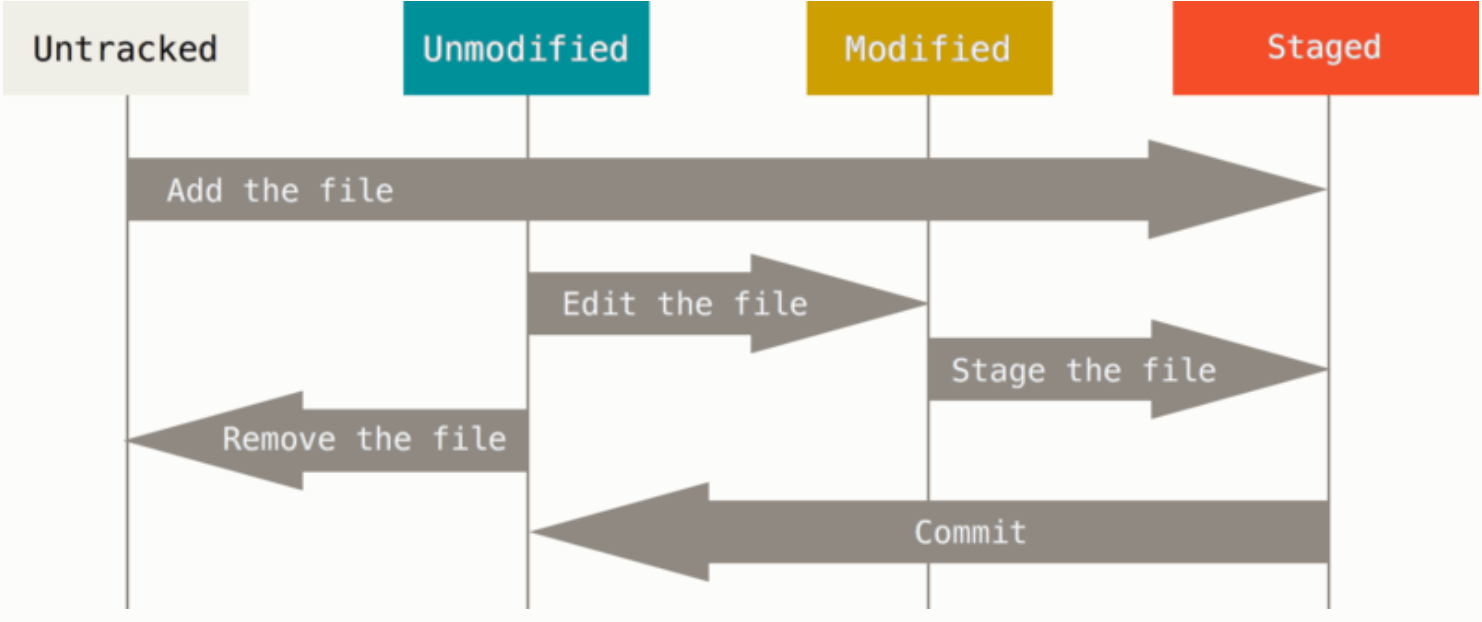
\includegraphics[width=0.75\textwidth]{fileLifeCycle.png}
    \attribution{https://git-scm.com/book/ru}
\end{center}

\subsection{Основные команды}

Для того чтобы добавить под версионный контроль новый файл, используется команда git add. Если файл уже и так под управлением Git, к следующему коммиту добавляются изменения относительно последнего коммита (то есть её название <<добавить>> относится не к файлам, а к сделанным изменениям, которые добавляются в индекс для последующего коммита, но и новый файл можно понимать как изменение --- с пустого файла до текущей версии). Так что в Git возможно часть изменений внутри одного файла закоммитить, а часть оставить на будущее --- файл при выполнении команды add копируется в staging area, и оттуда попадает в коммит, так что изменения после git add остаются только в рабочей копии.

Команда git status позволяет узнать, какие файлы в каком состоянии находятся. Для того чтобы узнать, что конкретно поменялось, а не только какие файлы были изменены, надо использовать команду git diff. Важно отметить, что git diff сама по себе не показывает все изменения, сделанные с последнего коммита --- только те, что еще не проиндексированы. Такое поведение может сбивать с толку, так как если сделать git add на все файлы, то git diff ничего не вернет (зато git status покажет, что они в статусе <<added>>).

Чтобы сделать коммит, нужно выполнить команду git commit (логично, не правда ли?). Если git commit делать без параметров, то она откроет текстовый редактор для ввода комментария к коммиту. По умолчанию это вполне может быть Vim, знаменитый текстовый редактор под Linux, знаменитый прежде всего тем, что из него не так просто выйти. Поэтому обычно пишут \verb|git commit -m"<комментарий к коммиту>"|. В случае с графическими клиентами всё обычно гораздо приятнее, но несколько более трудоёмко, поэтому я чаще коммичу из командной строки.

Комментарии должны быть осмысленными, потому что это единственный способ быстро понять, что было сделано в том или ином коммите. Т.е. если вы разрабатываете большую систему и хотите найти какой-то давний коммит, то это будет гораздо проще сделать просмотром лога коммитов с комментариями, чем диффов. Таким образом, коммиты с пустым или неадекватным текстом в комментарии в индустрии страшно караются. В комменте не нужно писать, какие файлы поменялись (это и так видно по диффу). Пишите, почему они поменялись --- что вы там сделали и зачем, как изменилась логика, что добавилось/удалилось (не какие строки, а в плане семантики) и т.п.

Для того чтобы удалить файл из Git, надо удалить его из отслеживаемых файлов (точнее, удалить его из индекса) а затем выполнить коммит. Это позволяет сделать команда git rm, которая по умолчанию также удаляет файл из рабочего каталога, но её можно попросить перевести файл в статус <<неотслеживаемый>>.

Историю коммитов позволяет увидеть команда git log. У нее есть много всяких параметров, которые позволяют красиво форматировать вывод истории. Например, можно сделать алиас на команду 

\begin{minted}{text}
git log --pretty=format:\"%h %ad | %s%d [%an]\" --graph --date=short
\end{minted}

который удобным образом показывает хэш и дерево коммитов, дату, комментарий и автора коммита. Всякие TortoiseGit позволяют рисовать красивые картинки. На GitHub тоже есть рисовалка дерева коммитов, во вкладке Insights репозитория.

Чтобы откатить локальные непроиндексированные изменения (поправили файл и поняли, что лучше бы этого не делать и вернуть как было), нужно выполнить команду \verb|git checkout <имя файла>| или, что более мнемонично, \verb|git restore <имя файла>|.

Ещё полезно знать команды, которые откатывают все изменения сразу. Прежде всего \verb|git reset --hard| --- по умолчанию восстанавливает все отслеживаемые файлы в состояние на момент последнего коммита. Однако неотслеживаемые файлы оно не трогает, и тут поможет \verb|git clean -dfx| --- команда, удаляющая все неотслеживаемые файлы из репозитория. Так что git reset и git clean вместе возвращают репозиторий в <<первозданное>> состояние, как после git clone, что очень удобно при отладке ошибок сборки.

\section{Git, установка и базовые операции}

\subsection{Установка}

Попробуем вместе с нуля всё поставить, создать локальный репозиторий, научиться коммитить, смотреть историю и откатывать изменения. Будем предполагать, что всё происходит на операционной системе Windows (на Linux на самом деле всё примерно так же, но даже проще) и будем считать, что менеджер пакетов Chocolatey по какой-то причине не используется.

Итак, сначала надо поставить консольный клиент Git. Скачиваем инсталляционный пакет с официального сайта (\url{https://git-scm.com/downloads}), выбираем там <<Click here to download>>, что должно начать скачивание 64-битной версии. Запускаем инсталлятор. Принимаем лицензию, кликаем Next, в меню <<Select components>> снимаем галочку <<Windows Explorer integration>> (мы планируем поставить графический клиент, так что довольно убогая функциональность Git по интеграции с файловым менеджером нам не понадобится --- тем более, мы, как настоящие программисты, должны пользоваться Windows Explorer очень редко). Жмём Next.

Дальше нам предложат выбрать текстовый редактор для редактирования сообщений о коммитах и прочих таких вещей. По умолчанию Vim, но я бы выбрал Visual Studio Code или Notepad++, или какой вам нравится из предложенного в инсталляторе списка. Вроде как надо, чтобы редактор у вас уже был установлен.

На следующей странице предлагается выбрать название ветки по умолчанию. Cancel culture добралась даже до Git, и историческое название основной ветки master было признано нетолерантным по отношению к афроамериканцам, долгое время страдавшим в рабстве. Сейчас принято называть главную ветку main, но по умолчанию всё-таки нетолерантное master.

На следующей странице оставьте по умолчанию <<Git from the command line and also...>> --- Git пропишется в системную переменную PATH и вы сможете вызывать его из консоли просто командой git, бе указания пути до того места, куда он поставился. На следующей странице оставьте <<Use bundled OpenSSH>> --- Git таскает с собой все зависимости, включая криптографическую библиотеку OpenSSH, которая ему нужна для работы с удалёнными репозиториями. То же с <<Use the OpenSSL library>> на следующей странице.

На следующей странице надо оставить по умолчанию, <<Checkout Windows-style, commit Unix-style line endings>>. Тут дело в том, что разные операционные системы используют разные признаки конца строки в текстовых файлах (человечество не может договориться даже в этом). В Windows это \verb|\r\n| --- перевод строки и возврат каретки, традиция, пошедшая от механических печатных машинок. В Linux это \verb|\n|, в macOS это \verb|\r|. Но исходники должны выглядеть на всех ОС одинаково, и переводы строк не должны считаться значимым изменением кода. Поэтому в Git по соглашению принято так: в репозитории все файлы хранятся в Linux-стиле, с \verb|\n| в качестве перевода строки, при получении файлов Git автоматически их конвертит в переводы строки, принятые в текущей операционной системе, при коммите конвертит обратно. Несоблюдение этого правила возможно, но может привести к ругани редакторов и некоторой боли, поэтому этого правила придерживаются, даже если разработка всегда идёт на одной ОС.

На следующей странице можно выбрать консоль, используемую Git, если его просто запустить из меню <<Пуск>>. MinTTY (по умолчанию) имеет более линуксовый стиль, но довольно удобна. cmd может быть привычнее, если вы и так пользуетесь консолью Windows. На самом деле, если вы всё делаете правильно, вы всё равно будете вызывать команды git из уже запущенного терминала, так что без разницы.

На следующей странице предлагается выбрать поведение команды git pull, которая получает изменения из удалённого репозитория. Поскольку, чтобы объяснить выбор, надо сначала рассказать про ветки и про удалённые репозитории, оставьте просто по умолчанию --- большинство проектов всё равно работают с pull именно так.

На следующей странице оставьте по умолчанию <<Git credential manager>> --- это интегрируемая в менеджер паролей Windows штука, которая позволит не вводить логин-пароль каждый раз при выкладывании изменений в удалённый репозиторий. Очень удобно. На следующей странице тоже оставьте настройки по умолчанию --- кеширование даст Git работать побыстрее за счёт большего расхода памяти (и то и то для нормальных проектов не заметно, поэтому не важно, но пусть будет), и символические ссылки можно не включать --- если у вас в репозитории они есть, то лучше просто уберите, это может быть удобно в Linux-проектах, и Windows умеет их поддерживать, но это всё ещё считается неким извращением.

На следующей странице можно оставить галочки про экспериментальные фичи выключенными, они нам всё равно не понадобятся пока.

Дальше жмём Install и ждём, пока всё поставится.

Теперь поставим графический клиент TortoiseGit\footnote{Под Linux его нет, но он там и не нужен особо --- пользователи Linux обычно и так привычны к консоли, обычного консольного клиента Git будет достаточно. Так что если у вас Linux, этот шаг можно пропустить.}. Идём на \url{https://tortoisegit.org/download/}, там качаем последнюю версию <<for 64-bit Windows>>. Инсталлятор, в отличие от Git, лишних вопросов не задаёт, так что кликаем Next несколько раз и ждём, пока поставится. Дальше жмём Finish, запускается First start wizard. Вот тут уже начинаются вопросы. Язык лучше оставить английский (надо привыкать), указываем путь до установленного Git (по умолчанию он сам найдёт, но можно нажать Check now, чтобы проверить, что путь правильный). 

Дальше указываем свои Name и Email, под которыми будете коммитить. Вот это довольно важная штука, потому что желательно, чтобы они совпадали с вашим аккаунтом на GitHub и почтой, на которую вы регистрировались (или зарегистрируетесь). Это не обязательно, но если это будет так, GitHub сможет правильно понимать авторство коммитов и показывать их в вашей статистике. Имя пользователя должно быть адекватным, никаких Nagibator666 --- желательно, чтобы имя пользователя содержало ваши имя и фамилию. Аккаунт на GitHub --- это важная часть резюме, он должен выглядеть профессионально. Вы можете думать, что пока можно под <<плохим>> аккаунтом посидеть, а потом, когда станете крутым специалистом, завести себе новый и хороший. Но практика показывает, что <<плохой>> аккаунт остаётся навсегда (что логично --- вряд ли кто, проснувшись поутру в один прекрасный день, осознаёт, что вот сегодня он уже крутой специалист и пора заводить новый аккаунт). Тем более что даже домашки, выложенные на GitHub, для HR-ов --- опыт программирования и <<стаж>> разработчика.

Остальное оставляем по умолчанию. После установки TortioseGit желательно перезагрузиться, чтобы он закончил интеграцию в Windows Explorer (без перезагрузки тоже будет работать, но может не отображать статусы файлов в рабочей копии или ещё что-нибудь такое).

\subsection{Работа с локальным репозиторием}

Теперь давайте создадим локальный репозиторий и попробуем с ним что-нибудь поделать. Для этого потребуется какая-нибудь пустая папка. Visual Studio, например, по умолчанию предлагает хранить код в папке пользователя/source/repos, так что и наш репозиторий можно создать там. Но вообще, конечно, где удобнее (в Linux обычно в домашней папке пользователя прямо). Итак, создаём пустую папку, тыкаем по ней правой кнопкой мыши, выбираем Git create repository here, жмём OK (обратите внимание, флажок <<Make it Bare>> выставлять не надо --- это репозиторий без рабочей копии, прежде всего для создания сервера). Если у вас нет TortoiseGit, просто переходим в созданную папку в консоли и пишем \verb|git init|.

В некогда пустой папке появилась скрытая папка .git, там, собственно, и хранится пока пустой репозиторий. Кстати, отображение скрытых файлов, расширений и т.п. должно быть включено в настройках отображения папок в Windows Explorer всегда, во избежание нелепых ошибок.

Создадим в этой папке какой-нибудь файл, например, program.c (просто как текстовый документ, потом после создания указываете ему расширение .c, открывать среду разработки или что-то пока не надо). Откроем его любым текстовым редактором (например, Visual Studio Code или даже просто блокнотом) и напишем там что-нибудь, например,

\begin{minted}{c}
int main(int argc, char* argv[])
{
    return 0;
}
\end{minted}

Файл сейчас не под управлением системы контроля версий (так что если мы сделаем git clean, он удалится). Добавим его. Если вы в консоли, то просто \verb|git add program.c|, через TortoiseGit --- правой кнопкой по файлу, TortoiseGit -> Add... -> ОК. По идее рядом с файлом должен появиться синий плюсик, означающий, что файл добавлен в индекс, но не закоммичен (если вы в TortoiseGit, конечно --- в консоли ничего интересного не увидите). Это соответствует Staged на картинке с фазами жизненного цикла.

Давайте закоммитим. Правой кнопкой по любому пустому месту внутри папки (обратите внимание, не по файлу), или поднимаемся на папку выше и кликаем по нашей папке с репозиторием. Жмём Git commit -> "master", появляется окно, где сверху поле для ввода комментария к коммиту, снизу список изменений, которые мы коммитим (в нашем случае это один добавленный файл). По файлам из списка изменений можно покликать двойным кликом, посмотреть дифф (что на самом деле рекомендуется делать перед каждым коммитом, чтобы случайно не закоммитить свой пароль от вконтакта или сквернословия в адрес препода\footnote{Видел такое, неоднократно.}. Вводим в поле Message что-нибудь разумное, описывающее назначение коммита, в повелительной форме, например, <<Add initial version of our program>>. Почему в повелительной --- комментарии к коммиту надо читать как <<If this commit will be merged into main branch, it will ...>>. Жмём <<Commit>>, жмём <<Close>>\footnote{Если вы в консоли, весь этот параграф сводится к git commit -m"Add initial version of our program", хотя сделать перед этим git status и git diff тоже нелишне.}. Рядом с файлом должен появиться зелёный кружок с галочкой (хотя я всегда выключаю отображение статусов, потому что ему всё равно нельзя доверять из-за кеширования статусов и долгой индексации, если репозиторий большой, и если репозиторий большой, индексация выполняется в фоне время от времени и ощутимо тормозит, заставляя тормозить весь компьютер).

Теперь давайте поменяем что-нибудь в файле. Например, так:

\begin{minted}{c}
#include <stdio.h>

int main(int argc, char* argv[])
{
    printf("%s", "Goodbye, cruel world");
    return 0;
}
\end{minted}

Закоммитим файл ещё раз. Так же, правой кнопкой по файлу, TortoiseGit -> Add, затем Git commit -> "master", вводим новое сообщение о коммите, например, <<Add greeting>>, жмём Commit и Close. На самом деле, TortoiseGit -> Add можно пропустить, TortoiseGit по умолчанию добавляет к коммиту все изменённые файлы, и при коммите можно галочками выбрать, какие файлы добавлять к коммиту, какие нет. Однако консольный Git ведёт себя не так, там надо обязательно сделать \verb|git add program.c|, затем \verb|git commit -m"Add greeting"|\footnote{Это не совсем правда, можно git add не делать, а сделать сразу git commit -a -m"Add greeting". Ключ <<-a>> как раз и означает <<добавить к коммиту все изменённые файлы>>, но в силу отсутствия интерактивности это плохая практика --- вы можете неожиданно для себя закоммитить то, что совсем не хотели. В отличие от TortoiseGit, где можно посмотреть список и выбрать нужное.}.

Теперь давайте посмотрим историю изменений нашего файла. Правый клик на свободное место в папке, TortoiseGit -> Show log. Появляется окно, где сверху графически отображается дерево коммитов (пока очень куцее, всего два коммита, и даже для настоящего репозитория чтобы это было дерево, надо поставить флажок <<All Branches>> внизу слева). Снизу отображается информация о коммите --- его SHA-1-хеш (это уникальный идентификатор коммита, по его хешу с ним можно делать что угодно), комментарий, ещё ниже --- список изменений в этом коммите (очень куцый, у нас поменялся всего один файл). Можно кликнуть на другой коммит, и потом на файл двойным кликом --- это покажет, что конкретно поменялось в выбранном файле в выбранном коммите.

А теперь давайте вспомним, что Git --- это машина времени, и откатим изменение последнего коммита, вернув репозиторий в состояние на момент добавления файла. Кликнем правой кнопкой на первый коммит, выберем <<Reset "master" to this>>, в Reset Type выберем <<Hard>>, нажмём OK. Теперь откроем program.c в текстовом редакторе и убедимся, что он вернулся в первозданное состояние. Второй коммит потерялся, кстати, поскольку ветка master на него больше не указывает, и так просто вернуться к нему нельзя. Впрочем, он ещё есть в репозитории, как <<висячий>> коммит, на который никто не указывает и который соберёт сборщик мусора рано или поздно (где-то через пару месяцев --- Git осторожен и не любит терять потенциально ценные данные). В этом можно убедиться правым кликом на папке, TortoiseGit -> Show RefLog, найти там последнее действие <<commit>>, увидеть комментарий ко второму коммиту. Кстати, правым кликом по действию мы можем вернуть master на этот коммит и тем спасти его от уничтожения, но не будем этого делать. Вообще, RefLog --- это журнал всех действий с ветками, так что если вы случайно потеряли коммит, удалили ветку или сделали ещё что-то противоестественное, RefLog вас может спасти. Однако если вы всё делаете правильно, RefLog вам не понадобится.

На этом первое знакомство с Git можно закончить и перейти к следующей важной штуке --- веткам.

\section{Работа с ветками}

Ветки позволяют истории разработки ветвиться и сливаться. Тот факт, что каждый разработчик в команде работает независимо, делает ветки на самом деле ключевой функциональностью Git --- каждый разработчик имеет свою ветку, в которой пишет код, а затем сливает её с основной, даже если не знает про ветки ничего. Зато если знает, он может завести себе несколько веток для нескольких разных фич (например, нескольких домашек) и вести разработку параллельно, не мешая самому себе. Или быстро поэкспериментировать с несколькими вариантами решения, гарантированно ничего не напортив. Или месяц пилить какую-то сложную фичу, не мешая двум важным релизам, запланированным на этот месяц.

Технически, ветка --- это цепочка коммитов. Ещё более технически, ветка --- это просто указатель на коммит. Каждый коммит (кроме первого) хранит в себе указатель на коммит-родитель (на основе которого он сделан), так что если мы знаем указатель на какой-то коммит, мы по цепочке указателей всегда можем дойти до самого первого коммита и получить текущую версию всех исходников. И уж совсем технически, поскольку Git использует SHA-1 хеши как имена файлов в репозитории (в папке .git), а в файлах в репозитории хранятся как собственно файлы исходников, так и сами коммиты, то указатель --- это просто SHA-1-хеш. Зная хеш, можно за константу (ну, почти --- со скоростью файловой системы) найти нужный объект.

Рабочая копия помнит <<текущую>> ветку, и когда вы делаете коммит, этот коммит запоминает предыдущий коммит этой ветки как своего родителя, затем текущая ветка перекидывается на новый коммит (почему, собственно, ветка master продвинулась, когда мы сделали второй коммит)\footnote{Кстати, в Git есть ещё тэги --- <<константные ветки>>, которые не продвигаются при коммитах, удобны для того, чтобы отметить/<<запомнить>> конкретный коммит.}. Можно завести новую ветку, тогда текущая ветка в рабочей копии переключится на неё и новые коммиты будут продвигать эту ветку, а не старую, делается это консольной командой \verb|git checkout -b <имя ветки>| или в TortoiseGit правой кнопкой по папке, TortoiseGit -> Create Branch. В TortoiseGit как обычно выбор больше --- помимо названия ветки можно указать, от какой ветки отводить (HEAD --- текущая ветка в рабочей копии, в скобках указано её название), можно отвести ветку от тэга или даже конкретного коммита. Не забудьте поставить галочку <<Switch to new branch>>, иначе ветка создастся, но рабочая копия останется на старой ветке, так что надо будет вручную переключиться на новую\footnote{Консольная команда git branch при создании ветки ведёт себя так же, потому я рекомендую несколько менее каноничную git checkout -b.}. Чтобы убедиться, что всё правильно, достаточно в консоли выполнить \verb|git status| --- первой строкой выдачи он напишет <<On branch имя-ветки>>; в TortoiseGit просто правый клик по папке отобразит в контекстном меню Git commit -> <имя ветки>. За этим надо внимательно следить, потому что очень много грустных историй начиналось с <<я случайно не в ту ветку закоммитил>>.

Переключение веток --- консольная команда \verb|git checkout <имя ветки>| или TortoiseGit -> Switch/Checkout. Она делает две вещи --- выставляет текущую ветку в рабочей копии на желаемую и обновляет файлы в рабочей копии так, чтобы они соответствовали состоянию ветки, на которую мы переключаемся. Обратите внимание, если в рабочей копии есть какие-то незакоммиченные изменения, которые при переключении будут затёрты изменениями из другой ветки, переключение будет невозможно. Git не даст потерять данные --- надо сначала сделать коммит в старую ветку, затем переключиться на новую. Впрочем, новые или изменённые файлы, которые коммиты из новой ветки не трогали, вполне ок --- они просто останутся изменёнными после переключения и их можно будет закоммитить уже в новую ветку, работа не потеряется.

Обратите внимание, ветки и папки в файловой системе никакого отношения друг к другу не имеют! Ветки --- это способ управлять изменениями, папки --- файлами. Можно это понимать, как два измерения --- файлы похожи на пространство, коммиты на время. Соответственно, папки в репозитории --- это пространственная группировка данных, ветки --- временная (те самые альтернативные ветки истории, про которые упоминалось в самом начале).

\subsection{Слияние}

Когда работа в ветке закончена (например, доделана большая фича), её надо влить в основную ветку. Для этого используется операция слияния. Делается она в два этапа --- сначала переключаемся на ту ветку, \emph{в которую} хотим влить изменения (например, командой \verb|git checkout master|), затем командой \verb|git merge <имя ветки>| перекладываем изменения из ветки, \emph{из которой} мы хотим их смерджить. При этом создаётся \emph{мердж-коммит} --- особый коммит, у которого два родителя: последний коммит из ветки, в которую мерджим, и последний коммит из ветки, из которой мерджим. И текущая ветка (в которую мерджим) переставляется на мердж-коммит, тем самым исходники в рабочей копии начинают включать в себя изменения, относящиеся как к одной ветке, так и к другой. 

Звучит сложно, но визуально может быть гораздо понятнее:

\begin{minted}{text}
    $ git checkout master
    $ git merge iss53
\end{minted}
\begin{center}
    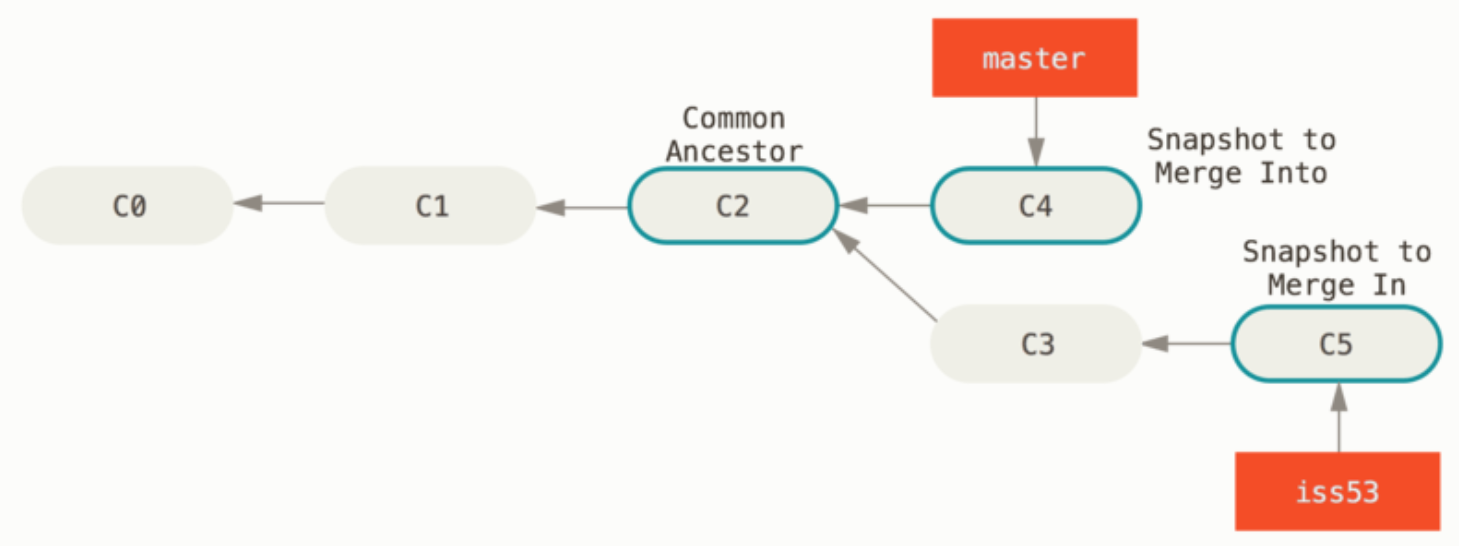
\includegraphics[width=0.7\textwidth]{merge.png}
\end{center}
\begin{center}
    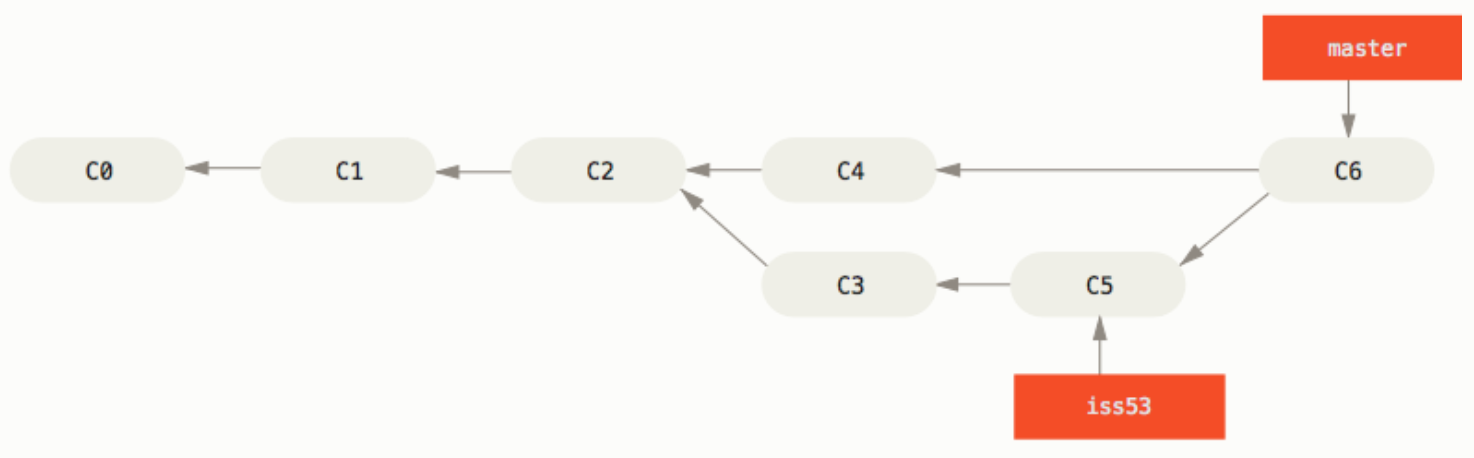
\includegraphics[width=0.7\textwidth]{mergeResult.png}
    \attribution{https://git-scm.com/book/ru}
\end{center}

В TortoiseGit всё так же --- переключаемся с помощью Switch/Checkout на ветку, \emph{в которую} хотим мерджить, делаем TortoiseGit -> Merge..., выбираем ветку, из которой хотим мерджить, оставляем галочки по умолчанию. Обратите внимание, мерджить из коммита --- это вмерджить не только этот коммит, а коммит и все его родительские коммиты до общего предка\footnote{Git умеет и отдельный коммит, командой git cherry-pick, но это чёрная магия.}.

Обратите внимание, что у веток обязательно должен быть общий предок, иначе мердж вообще невозможен. А ещё у мердж-коммита обычно нет осмысленного комментария, потому что это чисто техническая вещь.

\subsection{Конфликты}

Естественно, в реальной разработке чистый мердж --- это большая редкость. Чаще всего имеются конфликты --- когда изменения в обеих ветках затрагивают одно и то же место. Обратите внимание, что если даже изменения в двух ветках были в одном файле, но в разных его местах, Git смерджит такой файл самостоятельно и конфликта не возникнет; проблема возникает только в том случае, когда Git без посторонней помощи не может решить что делать --- то ли в одной из веток код свежее и надо взять его, то ли надо взять оба варианта и расположить первый под вторым или второй под первым. В таком случае решение предлагается принять разработчику. Создаётся временная ссылка MERGE\_HEAD, указывающая на ветку, из которой мы мерджим изменения, и для каждого файла с конфликтом создаётся ещё два файла --- как было в HEAD, как было в MERGE\_HEAD, и как теперь. <<Как теперь>> содержит маркеры \verb|<<< === >>>|, обозначающие места с конфликтами, специально, чтобы код не скомпилировался:

\begin{center}
    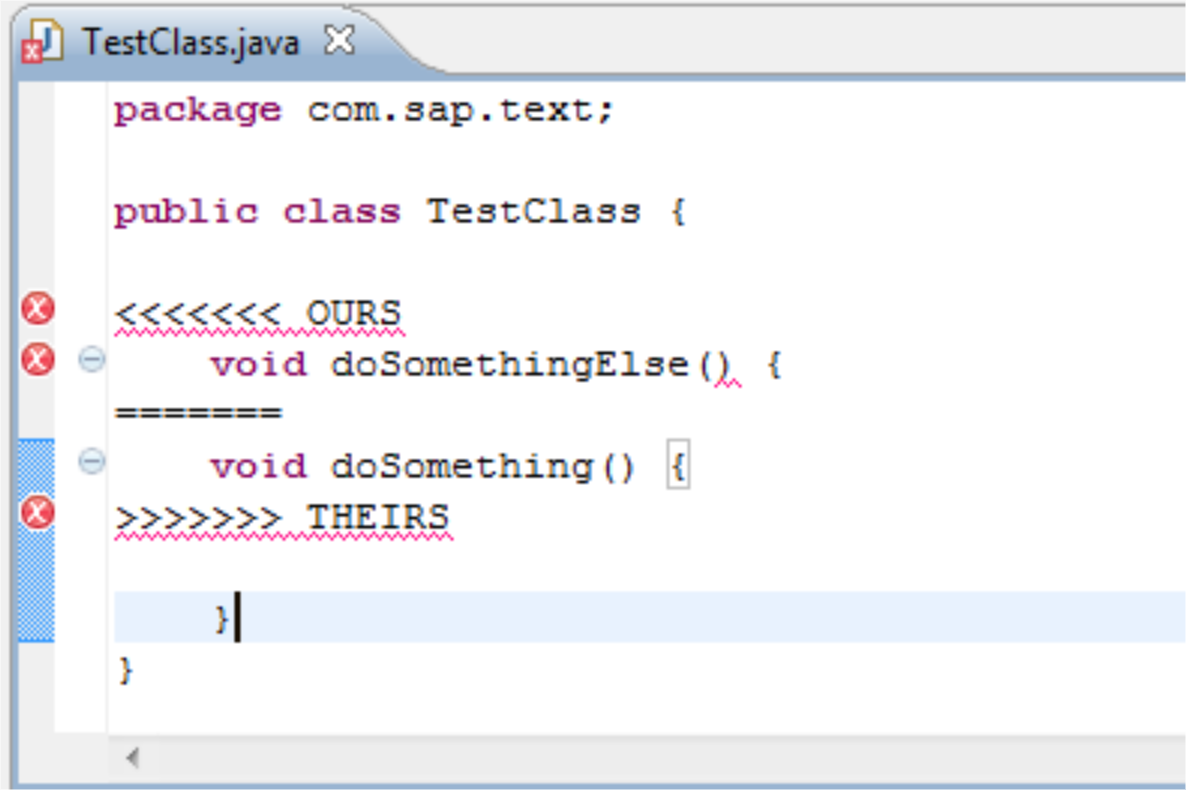
\includegraphics[width=0.4\textwidth]{conflictsInCode.png}
\end{center}

Хорошая новость в том, что большинство графических инструментов умеют показывать и редактировать конфликты красиво и удобно. Например, в TortoiseGit это выглядит так:

\begin{center}
    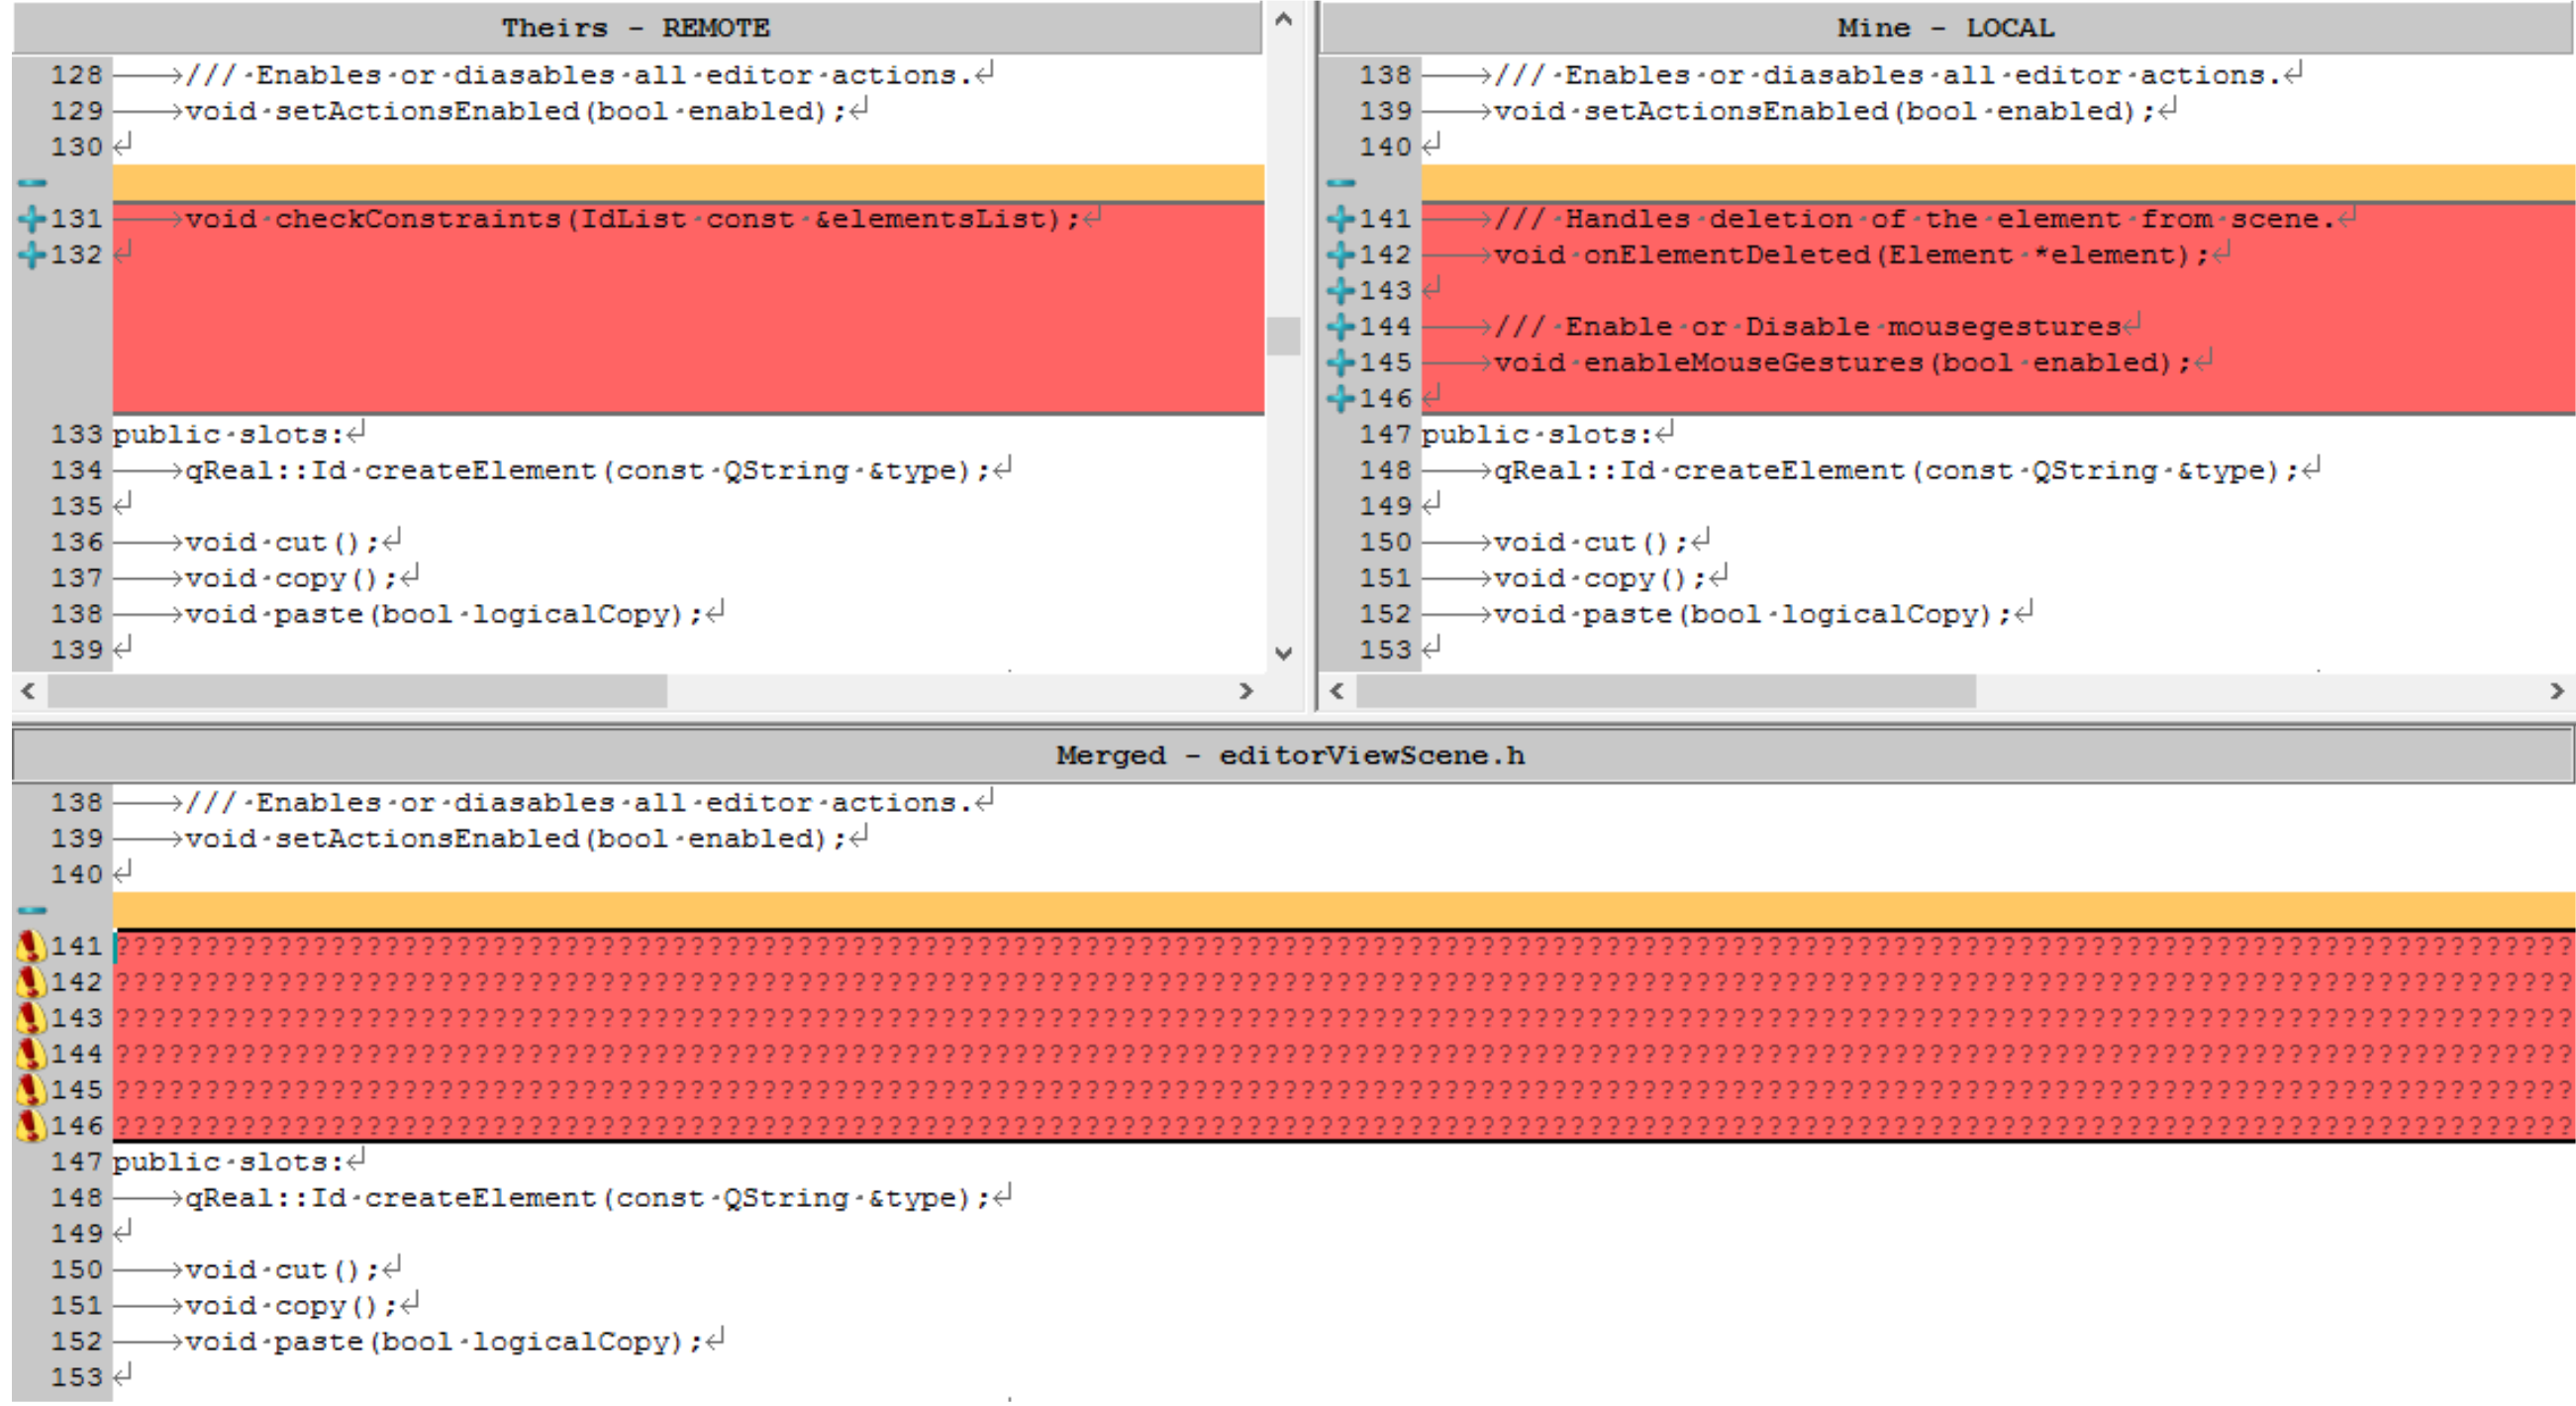
\includegraphics[width=0.95\textwidth]{conflicts.png}
\end{center}

Если вы поняли, что с конфликтами не разобраться (например, при мержде ветки, которая была в работе пару месяцев, конфликты могут быть в паре тысяч файлов, а вам надо срочно пофиксить баг), надо сделать 

\begin{minted}{text}
$ git merge --abort
\end{minted}

Эта команда попытается восстановить состояние рабочей копии на момент до мерджа (ей может не удасться, если после мерджа были изменения). Если вы удовлетворены процессом мерджа, надо сделать коммит, но не писать комментарий --- для мердж-коммитов комментарий сгенерируется автоматически. Если вы сделали мердж-коммит, но потом начали об этом жалеть, то поможет git reset или соответствующие манипуляции с логом в TortoiseGit, как было описано в туториале. Если откатить merge commit, то с точки зрения Git мерджа словно бы и не было.

Кстати, мердж имеет один специальный случай --- fast-forward. Это когда делается мердж с веткой, которая уже содержит все наши коммиты (например, когда делаете git pull, придя утром на работу и не успев ещё ничего написать). В таком случае ветка просто продвигается до той, которую вы мерджите, никаких попыток посчитать диффы и найти конфликты не делается (что логично, это ведь просто перестановка указателя на коммит), мердж-коммит тоже не создаётся.

\section{Работа с удалёнными репозиториями}

Для совместной разработки с Git настраивают один или несколько удалённых репозиториев (как правило, в каком-нибудь облачном сервисе типа GitHub или BitBucket, но часто корпоративная политика безопасности заставляет настроить репозиторий в локальной сети). Поскольку Git --- распределённая система, все репозитории технически равноправны и обмениваются изменениями (на самом деле коммитами). Однако каждый репозиторий в Git может иметь ссылку на репозиторий, с которого он был склонирован --- она называется \emph{origin}. Помимо этого, можно вручную добавлять и удалять ссылки на другие репозитории, в терминологии Git \emph{ремоуты} (от англ. remote) --- просто именованные URL репозитория. Все команды для работы с удалёнными репозиториями могут принимать нужный ремоут как параметр и используют ремоут origin по умолчанию.

Чтобы просмотреть, какие удалённые репозитории знает ваш локальный репозиторий, есть команда git remote (или в TortoiseGit это Settings -> Git -> Remote). Для репозитория, созданного командой git init (как в нас в туториале) список будет пуст --- наш репозиторий ни про кого не знает.

Чтобы склонировать чужой репозиторий, используется команда git clone (Git Clone... в TortoiseGit). Она работает \emph{только вне} существующего репозитория, так что если хотите что-то склонировать, поднимитесь на папку выше той, в которой делали репозиторий в туториале. Можно попробовать склонить, например, исходники Git с GitHub: \url{https://github.com/git/git}. Кликаем на GitHub на большую зелёную кнопку Code, копируем ссылку (\url{https://github.com/git/git.git}) и, у себя на локальном компьютере тыкнув правой кнопкой на пустом месте в папке выше нашего тестового репозитория, выбираем Git Clone. В качестве URL сама подставится из буфера обмена скопированная нами ссылка \url{https://github.com/git/git.git}, в поле Directory само же заполнится как, например, \verb|C:\Users\yurii\source\repos\git|, жмём на ОК и ждём, пока репозиторий склонируется. Чтобы не ждать очень уж долго (ведь клонируется весь репозиторий, со всей историей разработки Git с 2005-го года), можно поставить галочку Depth и установить её в 1 --- тогда история копироваться не будет, сервер просто отдаст текущее состояние исходников, что полезно, чтобы просто посмотреть. Перейдя к свойствам репозитория (Settings -> Git -> Remote) можно увидеть ремоут origin.

Когда вы хотите поделиться своими наработками\footnote{Давайте не будем делиться наработками с репозиторием Git (можете попробовать, но просто не пройдёте авторизацию) --- буквально через пару страниц мы создадим свой удалённый репозиторий на GitHub.}, надо отправить (push) их в главный репозиторий. Команда для этого действия --- git push в консоли или Git Sync... -> Push в TortoiseGit. При пуше можно выбрать ремоут, в который мы пушим (обычно в origin, но можно в любой другой), и ветку, локальную и удалённую, из которой и, соответственно, в которую мы хотим запушить. Обратите внимание, что как правило имена локальной и удалённой веток совпадают, но это разные ветки, с потенциально разными коммитами и потенциально разной историей.

Из консоли всё работает так же, но проще:

\begin{minted}{text}
$ git push origin master
\end{minted}

Или просто

\begin{minted}{text}
$ git push
\end{minted}

По умолчанию в качестве ремоута используется origin, а в качестве ветки --- так называемая отслеживаемая ветка. Для каждой ветки локального репозитория можно задать ветку в удалённом репозитории, в которую будут пушиться изменения по умолчанию. Когда репозиторий клонится, для каждой удалённой ветки создаётся локальная ветка и отслеживаемая ветка для каждой локальной устанавливается в соответствующую удалённую. Когда вы создаёте ветку в локальном репозитории, удалённый про неё ничего не знает, поэтому надо при первом пуше из неё явно указать, куда пушите и выставить отслеживаемую ветку. В консоли --- командой \verb|git push -u origin <локальное имя ветки>:<удалённое имя ветки>|\footnote{Ключ -u имеет полную форму c более говорящим названием \mintinline{text}{--set-upstream}.}, в TortoiseGit через Git Sync... -> Push. Если в удалённом репозитории появилась ветка, про которую локальный ничего не знает, то надо сначала её подтянуть командой git fetch (вообще, git fetch получает все изменения во всех ветках, но не трогает рабочую копию) и потом переключиться на неё с помощью git checkout или аналогичной командой в графическом клиенте. Обратите внимание, в вашем локальном репозитории хранятся удалённые ветки, локальные ветки, трекающие удалённые, и ещё есть удалённый репозиторий, в котором есть настоящие удалённые ветки. И поскольку удалённый репозиторий может меняться без вашего участия (например, сокомандниками), то состояние всех этих веток может отличаться! Звучит сложно, но на практике умолчания настолько удобны, что кажется, что Git всё делает за вас. По крайней мере, бывают профессиональные разработчики, которые не знают, чем pull от fetch отличается.

Ну и, наверное, все уже догадались, что команда git pull (или Git Sync... -> Pull в TortoiseGit) притягивает изменения из удалённой ветки в локальную. То есть по сути push наоборот. Каждый рабочий день любого нормального программиста обычно начинается с git pull, чтобы получить самую свежую версию исходников. Pull обновляет в репозитории состояние текущей ветки и мерджит изменения из удалённого репозитория, если они были, в локальную ветку. Разумеется, чистый мердж --- редкость и означает, что либо вы, либо ваши сокомандники ничего не делали, так что при pull-е могут быть конфликты, которые надо разрешить. Плюс к тому, как обычно, если в рабочей копии есть незакоммиченные изменения, которые могут быть затёрты при pull-е, операция завершится с ошибкой, чтобы не потерять работу.

Симметрично, если в удалённом репозитории есть изменения, которых нет у вас, то push завершится с ошибкой (даже если можно чисто смерджится --- Git понимает, что какие-то изменения вы не видели, следовательно, не тестировали, будут ли ваши работать с ними). В таком случае надо сначала сделать git pull, при необходимости разобрать конфликты, а уже потом делать git push (если ваши коллеги не успели выложить что-то ещё, тогда процесс надо начинать сначала). А ещё pull можно делать практически откуда угодно, а вот push требует прав на запись в репозиторий --- по умолчанию они есть только у создателя репозитория.

Вот картинка, обобщающая и поясняющая операции с удалёнными репозиториями:

\begin{center}
    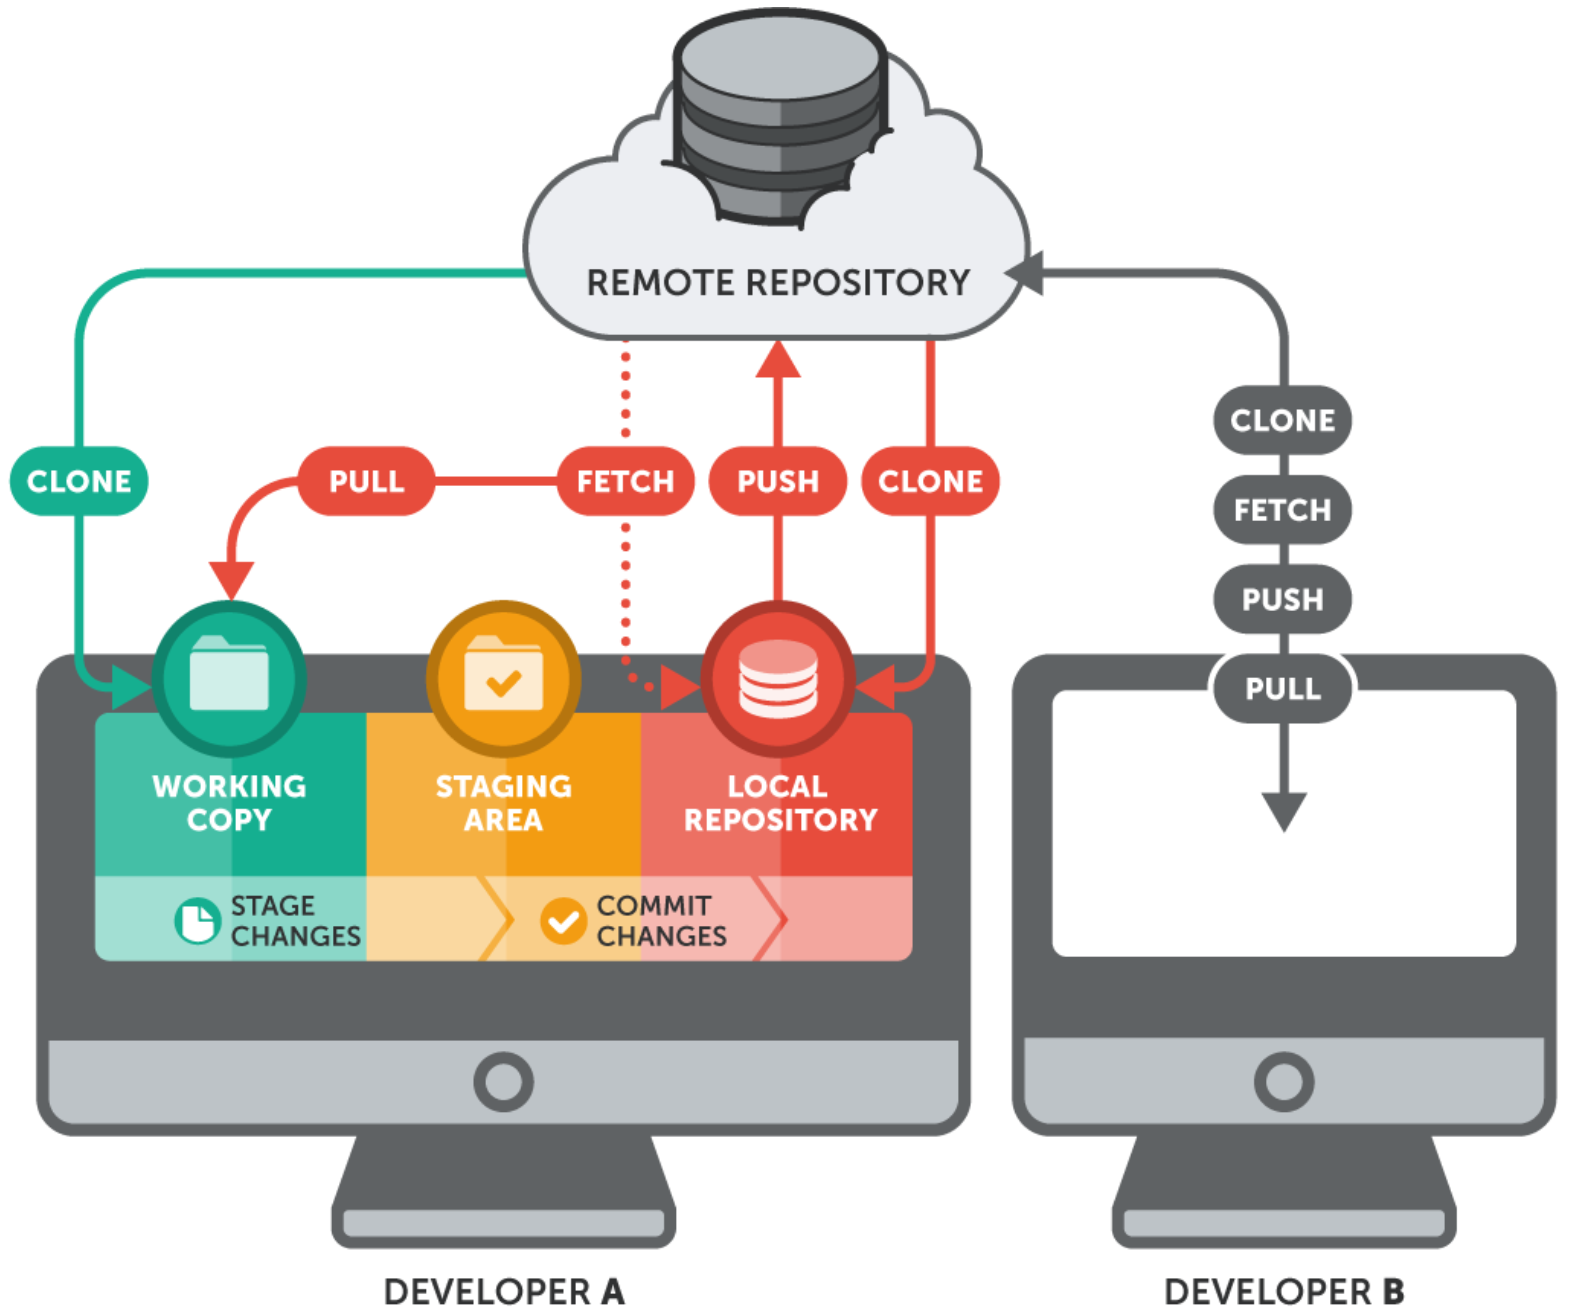
\includegraphics[width=0.8\textwidth]{remoteRepos.png}
    \attribution{https://www.git-tower.com/learn/git/ebook/en}
\end{center}

\section{GitHub}

Git полезен и сам по себе, но гораздо более полезен он как средство координации между членами команды. Для этого можно использовать как <<голый>> сервер, запущенный на какой-нибудь машине, видимой по сети, так и один из облачных сервисов, таких как GitHub, BitBucket, GitLab, Azure DevOps Server и т.п. Облачные сервисы, помимо хостинга репозитория, предоставляют ещё и удобный графический интерфейс для просмотра исходников и кучу дополнительной полезной функциональности для управления проектом или его сопровождения. Кстати, чтобы получить всё это, не обязательно пользоваться именно развёрнутым в облаке решением --- например, у GitLab есть self-hosted-версия, которую можно запустить у себя, и получить красивый интерфейс для работы с репозиторием, ничуть не хуже GitHub-а и не зависящий от санкций и других проявлений воли третьих лиц. Однако GitHub сейчас де-факто лидирует среди конкурентов, и большая часть мирового программного обеспечения с открытым исходным кодом разрабатывается с его помощью, а если не разрабатывается, то имеет зеркало с обновляемыми исходниками. Поэтому поговорим про GitHub подробнее.

Итак, помимо хостинга репозиториев GitHub умеет:

\begin{itemize}
    \item красивый UI для просмотра исходников и поиска по ним, с синтаксической подсветкой;
    \item пуллреквесты, то есть <<просьбы смерджить изменения оттуда-то>>, с хорошей функциональностью комментирования кода;
    \item форки --- клоны репозитория, которые можно делать прямо из веб-UI;
    \item социальное взаимодействие --- аккаунты с их оформлением, звёзды, наблюдаемые репозитории, организации;
    \item свою довольно крутую систему CI/CD --- GitHub Actions, и даже свой репозиторий пакетов, куда можно публиковать результаты сборки;
    \item средства для управления проектом --- GitHub Projects, вики (что интересно, вики репозитория на GitHub --- сами по себе Git-репозиторий), багтрекер.
\end{itemize}

И главное, всё это бесплатно для проектов с открытым исходным кодом.

\subsection{Туториал, работа с GitHub}

Давайте попробуем выполнить первые шаги любого нормального проекта с открытым исходным кодом.

Первое, что нудно сделать --- если у вас нет аккаунта на GitHub, завести его. Для этого потребуется нормальная почта, поэтому если есть только \verb|nagibator666@mail.ru|, сначала следует завести нормальную почту. Потом придумать себе хороший юзернейм --- лучше, если он будет содержать в себе имя и фамилию (например, yurii-litvinov), в любом случае он должен выглядеть максимально профессионально. Дальше идёте на \url{https://github.com/} и... регистрируетесь.

После регистрации у вас появляется страница с профилем, примерно вот такая: \url{https://github.com/yurii-litvinov}. Там есть вкладка <<Repositories>>, а на ней --- большая зелёная кнопка <<New>>. Кликаем на неё, появляется форма создания репозитория.

\begin{itemize}
    \item Имя репозитория --- тут, думаю, всё понятно, но опять-таки, оно должно быть адекватным.
    \item Описание --- пара предложений, про что проект.
    \item Публичный/приватный репозиторий --- приватные репозитории тоже бесплатны, но мы-то за открытый исходный код, поэтому если нет веских причин для обратного, выбираем Public. И нет, <<мне стыдно выкладывать свой код>> --- \emph{не} веская причина, его всё равно никто смотреть не будет, скорее всего. На GitHub миллионы репозиториев. Да даже если и будет, профиль, где есть старые репозитории с плохим кодом и новые с хорошим, для трудоустройства гораздо более полезен, чем профиль, где только новые с хорошим.
    \item Галочку <<Add a README file>> надо поставить, README в любом нормальном репозитории должен быть, и там должно быть написано, про что вообще этот проект, как его собрать и запустить (в подробностях, чтобы совсем сторонний человек мог воспроизвести). Туда же добавляются плашки от CI-системы, про которые будет дальше в курсе.
    \item Add .gitignore тоже надо выбрать, из набора шаблонов, соответствующих популярным средам разработки и языкам. Например, если планируете вести разработку на Kotlin, есть готовый файл .gitignore для него. Если вы не знаете, что такое .gitignore, буквально через пару страниц про него будет.
    \item Choose a license --- лицензия тоже обязательно должна быть. По умолчанию (если лицензии в репозитории нет) по международному и российскому законодательству об авторском праве вашим кодом никто не может пользоваться, даже если он лежит в общем доступе. Лицензия, собственно, и нужна для того, чтобы явно передать часть прав на интеллектуальную собственность, например, право использовать ваш код в чужом проекте. Желательно использовать какую-нибудь разрешающую лицензию, например, Apache License 2.0, MIT License, одну из BSD. Знаменитая GPL, хоть и является популярной для лицензирования открытого кода, нежелательна --- она требует, чтобы код, использующий ваш проект, сам был под GPL\footnote{Есть тонкости --- например, LGPL не требует этого, если вы просто линкуетесь к библиотеке, не меняя её.}, что делает такой код бесполезным для большинства коммерческих проектов\footnote{Опять-таки, тонкости --- именно <<для большинства>>, GPL не запрещает зарабатывать деньги, она просто требует, чтобы покупатель получал с программой и её исходники.}.
\end{itemize}

Кликаем на Create Repository, получаем через некоторое время пустой репозиторий, в котором уже есть файлы .gitignore, README.md и LICENSE. Его можно к себе склонить, кнопкой Code, копированием ссылки оттуда в TortoiseGit -> Git Clone... в чистой папке (либо из консоли, \verb|git clone <URL> <путь до папки, куда копировать — по умолчанию это имя репозитория>|), так же как выше клонили репозиторий с Git.

Теперь давайте просимулируем типичный сценарий работы над домашкой. Берясь за новую задачу, первое, что нужно сделать --- отвести ветку от master (или main). Кликаем по репозиторию, TortoiseGit -> Create Branch..., вводим какое-нибудь адекватное имя ветки, отражающее её назначение (<<homework1>>, например --- лучше по-английски и без пробелов, хотя формально Git не против любого названия), \emph{проверяем ещё раз, что отводим ветку от главной} (это в Base On, и это важно, потому что в диффе потом, когда вы сделаете пуллреквест, будут изменения относительно целевой ветки. Так что если вы отведёте ветку <<homework2>> от <<homework1>>, а не от main, то в пуллреквест ко второй домашке попадут изменения из первой, за что препод скажет всё переделать. В реальных проектах за пуллреквест пяти фич вместо одной тоже никто спасибо не скажет). Не забываем флажок Switch to new branch. Жмём на OK.

Теперь <<делаем в новой ветке домашку>>. Для демонстрационных целей можно просто создать проект в вашей любимой среде разработки, написать что-то вроде Hello, world, и этого будет достаточно. Дальше коммитим все изменения (это мы уже умеем из прошлого туториала). Дальше пушим --- правой кнопкой по папке с репозиторием, Push. Скорее всего, вас попросят авторизоваться, вводите те самые логин и пароль, которые указывали при регистрации на GitHub. Дальше по идее Credentials Helper их запомнит и вводить больше не потребуется, но забывать пароль от GitHub всё равно не стоит.

Теперь идём на GitHub в наш новый репозиторий. Там над списком файлов по идее должна была появиться плашка, что появилась новая ветка, не хотите ли Compare and pull request. Если нет, ещё выше есть вкладка Branches, там можно просмотреть все ветки вообще, и из каждой открыть пуллреквест кнопкой New pull request. Указываете название и описание пуллреквеста (если в нём всего один коммит, то название и описание заполняются автоматически по комментарию к коммиту, если больше --- надо проявить креативность и описать, что за пуллреквест). Проверяете (обязательно) дифф ниже --- в пуллреквесте должны быть только те изменения, которые к нему относятся, не должно добавляться каких-то непонятных файлов, не должно быть забыто нужных файлов. Если всё ок, жмём на большую зелёную кнопку, пуллреквест создан.

Новый пуллреквест появится на вкладке Pull requests в репозитории, и ссылку на него (например, \url{https://github.com/REAL-NET/Repo/pull/2}) можно отправлять на ревью (а можно при создании пуллреквеста назначить ревьюера, и тогда GitHub сам пришлёт ревьюеру нотификацию). Ревьюер комментит пуллреквест, вы исправляете замечания, делаете новые коммиты в ту же ветку, откуда был открыт пуллреквест, пуллреквест сам собой обновляется (на самом деле просто потому, что пуллреквест открывается из ветки, а не конкретного коммита --- все коммиты в эту ветку будут видны в пуллреквесте после его открытия). Когда ревьюер одобряет пуллреквест (жмёт в Review changes на Approve), вы мерджите пуллреквест просто большой зелёной кнопкой, прямо из интерфейса GitHub.

Поскольку может быть открыто сразу несколько пуллреквестов (каждый из своей ветки), то можно одновременно сдавать несколько домашек/делать несколько фич, каждую в своей ветке.

\subsection{Процесс работы}

Общий процесс командной разработки с GitHub (и не только с GitHub) выглядит так:

\begin{itemize}
    \item Программист хочет сделать новую фичу.
    \item Для неё он отводит себе ветку от main-а (или текущей основной ветки проекта, это не обязательно main, но об этом чуть позже).
    \item Реализует в новой ветке фичу.
    \item Тестит и рефакторит её, а когда считает, что она готова, делает пуллреквест.
    \item Пока пуллреквест ревьюят, программист делает новую фичу (опять-таки, отведя новую ветку от main-а).
    \item По пуллреквесту появляются замечания, программист переключается на ветку пуллреквеста и правит там замечания.
    \item Когда поправил, коммитит и пушит исправления, они автоматом добавляются в пуллреквест.
    \item Просит ревьюеров, чтобы они посмотрели фиксы.
    \item Переключается обратно на свою рабочую ветку и продолжает писать код, возможно, делая ещё пуллреквесты.
    \item Цикл повторяется до тех пор, пока пуллреквест не принимают.
    \item Программист удаляет ветку с фичей, когда она замерджена.
\end{itemize}

Так же выполняется работа и с домашками, только каждая фича --- это отдельная задача.

Помимо веток с фичами в реальных проектах часто ещё имеются следующие сорта веток:

\begin{itemize}
    \item разработческая (обычно называется develop) --- самые актуальные и, возможно, нестабильные исходники, именно от неё, а не от main, отводят ветки для новых фич, туда же делаются пуллреквесты из веток с фичами;
    \item main (или master) в этом случае играет роль стабильной ветки, где лежит протестированная и готовая к работе версия --- пользователь выполнив git clone и собрав проект, получает что-то, чем может непосредственно пользоваться;
    \item релизные ветки отводятся от develop для каждого релиза, чтобы процессу тестирования и багфиксов не мешала разработка новой функциональности; когда релиз готов, изменения мерджатся в main, багфиксы также по мере готовности мерджатся в develop;
    \item если в уже выпущенном релизе выявляются критические баги, от коммита с релизом в main отводятся хотфиксовые ветки --- в них баги фиксятся, и как только всё готово и протестировано, изменения перекладываются обратно в main (и, конечно, в develop);
    \item main размечается тэгами, соответствующими релизам, чтобы хотфиксы было понятно на каком коммите базировать.
\end{itemize}

На картинке это может выглядеть как-то так:

\begin{center}
    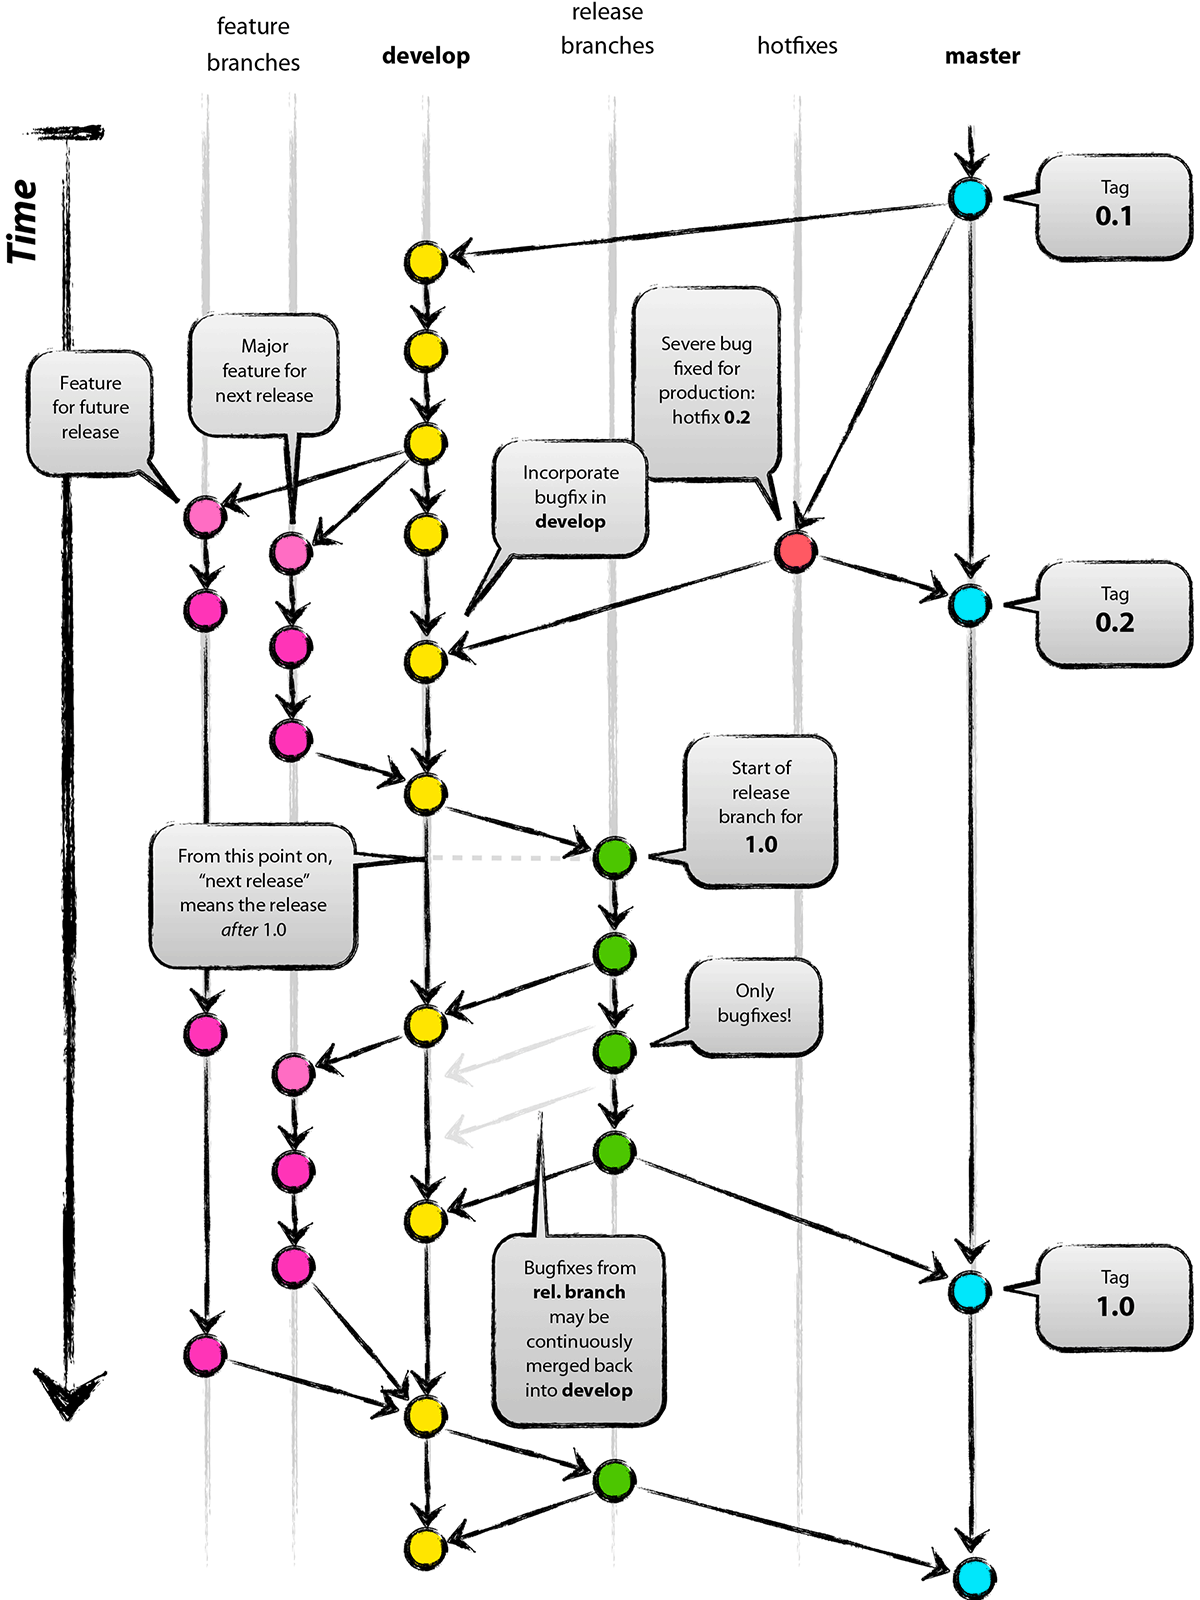
\includegraphics[width=0.6\textwidth]{gitFlow.png}
    \attribution{https://nvie.com/posts/a-successful-git-branching-model/}
\end{center}

Это довольно стандартный способ организации веток в репозитории, поэтому имеет своё название --- Git Flow.

\section{Хорошие практики}

Вот некоторые общеупотребимые практики при работе с системами контроля версий вообще и с Git в частности.

\begin{itemize}
    \item Коммитим только исходные тексты, конфиги, картинки и т.п. Следует избегать исполнимых файлов или слишком больших нетекстовых файлов, потому что для них дельту не посчитать, так что Git каждую версию вынужден хранить и передавать целиком.
    \item Если что-то может быть автоматически сгенерировано по тому, что уже есть в репозитории, это не надо коммитить. Потому что незачем, правильнее настроить автоматическую сборку так, чтобы это появлялось само у пользователя на машине.
    \item Всегда и обязательно пишем адекватные комментарии к коммитам. Обычно комментарий --- это одно-два полных осмысленных предложения (в повелительной форме, в духе <<Add ...>>, <<Fix ...>> и т.п.), описывающих, что же было добавлено в проект предлагаемыми изменениями. Причём, не какие файлы (это и так видно в логе), а что по сути --- фичи, фиксы багов (обязательно со ссылкой на нужный баг) и т.д. Комментарии типа <<fix>> или <<.>> могут быть поводом для брутального увольнения.
    \item Коммитим как можно чаще. Сделали что-то осмысленное --- коммит. Единственное требование --- чтобы закоммиченный код компилировался, чтобы коллегам не приходилось разбираться, кто сломал билд и что с этим делать. Ваш код может не работать, но не должен блокировать работоспособность остальной программы (например, вполне ок поместить его в большой if, включаемый параметром в конфиге).
    \item Никогда не коммитим исполнимые файлы (включая .dll/.so), объектные файлы, локальные настройки. Особенно исполнимые файлы --- выложить вирус в репозиторий кажется довольно глупым, но такое случалось пару раз на практике автора. Бывает так, что внешние зависимости выкладываются как бинарники (например, библиотеки для C++), потому что у них у самих куча зависимостей и собирать их в обычной сборке --- очень сложно и долго, так что из этого правила бывают исключения. Но если хотите так делать, надо чётко понимать альтернативы (скачивать при сборке с сетевого ресурса, например) и чётко знать, что и зачем вы делаете.
    \item Надо обязательно выкладывать все файлы, необходимые для сборки, не только исходники. Например, Проектные файлы, мейкфайлы, скрипты и т.п. Для Visual Studio это, например, .vcxproj и .sln, для IntelliJ IDEA, Rider и прочих IDE этой серии --- всё содержимое папки .idea, кроме workspace.xml и tasks.xml.
    \item Имеет смысл проверить, что всё в порядке, склонив свой репозиторий в пустую папку. Если всё соберётся одной консольной командой или парой кликов мышью, значит, всё ок.
    \item Кстати, никто не запрещает иметь локально несколько копий репозитория, например, с разными ветками. Просто разложите их по разным папкам и время от времени синхронизируйте командами push/pull с репозиторием на GitHub. Может быть удобно, если часто приходится переключаться между ветками, но может быть неудобно, если вы работаете над реальным проектом и код в собранном состоянии занимает 20 гигабайт, а у вас всего 128 гигабайт на рабочей виртуалке.
    \item Коммит не должен содержать в себе файлы, не относящиеся к изменениям. Поэтому нежелательно пользоваться ключом -a к git commit, очень желательно иметь правильный .gitignore и обязательно перед коммитом проверять, что же вы коммитите (git status как минимум, git diff желательно). То же касается пуллреквестов --- никогда не ленитесь смотреть diff.
    \item Коммит не должен добавлять/убирать пустые строки, менять пробелы на табы и т.д., если это не суть коммита. Такого рода изменения надо делать отдельными коммитами, иначе изменений по существу не будет видно в диффе.
    \item Стиль исходного кода и отступов должен совпадать с текстом вокруг. Особенно это касается больших проектов, надо обязательно либо прочитать местный стайлгайд, либо посмотреть на соседний код. Со своими порядками в чужой монастырь не ходят, сколь бы разумными вам ни казались эти порядки.
\end{itemize}

И главное правило, весь код, не запушенный на GitHub, не существует. Поэтому:

\begin{center}
    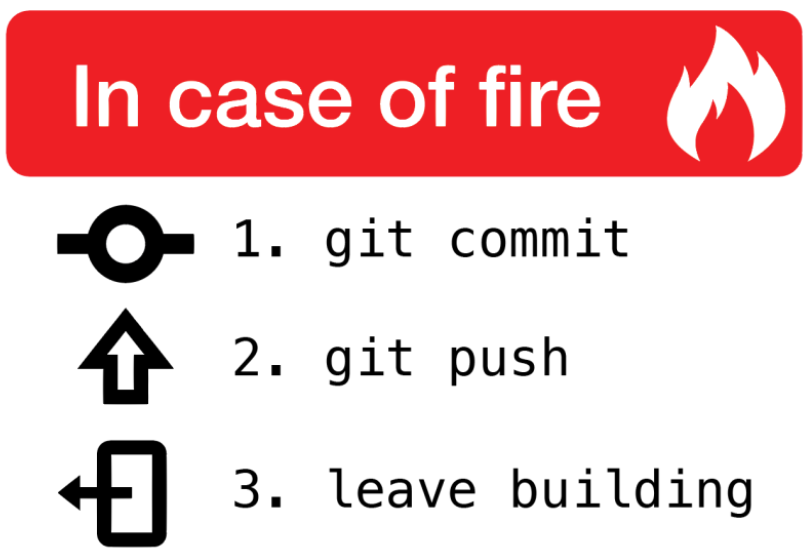
\includegraphics[width=0.3\textwidth]{inCaseOfFire.png}
    \attribution{Народная мудрость}
\end{center}

Серьёзно, с локальной машиной может случиться столько всего, что даже день работы держать только у себя на жёстком диске должно быть страшно. Выкладывайте всё, что хоть немного было бы обидно потерять.


\section{Ещё полезные команды}

Наконец, ещё несколько полезных штук, которые не очень известны, поэтому о них часто даже не догадываются:

\begin{itemize}
    \item \verb|git add -p| --- интерактивное добавление изменений к коммиту, позволяет коммитить только часть файла;
    \item \verb|git commit --amend| --- исправить последний коммит. Например, \verb|git commit --amend -m "an updated commit message"| обновит сообщение у последнего коммита. Однако применять git amend можно \textbf{только до} git push. Изменение уже опубликованной истории коммитов может иметь ужасные последствия --- коммит идентифицируется своим хешем, который считается от любой информации в коммите, так что после amend у вас локально и удалённо будут два совершенно разных с точки зрения Git коммита с одинаковым содержимым, что гарантирует конфликт при мердже.
    \item \verb|git reset --hard| --- откатить все изменения в рабочей копии до последнего коммита. Это не то чтобы малоизвестная команда, но очень полезна, особенно если вы всё испортили. Обязательно проверяйте git status, что не откатите лишнего.
    \item \verb|git reset --hard <хеш коммита>| --- откатить все изменения в текущей ветке до указанного коммита, забыть все коммиты, что были после (и случайно грохнуть всю домашку перед зачётом). В качестве хеша коммита может быть и ссылка, так что у этой команды есть одна часто применяемая форма: \verb|git reset --hard origin/master| --- откатиться до состояния, в котором находится код в удалённом репозитории. Так можно вылечить большинство проблем с тем, что вы что-то сделали не так и теперь в рабочей копии всё плохо.
    \item Все команды, которые могут испортить историю, делаются с ключом --force (или -f). Например, как откатить ветку до нужного коммита и выложить на GitHub:
        \begin{minted}{text}
git reset --hard <хеш нужного коммита>
git push -f origin <имя ветки>
        \end{minted}
        Без ключа -f Git резонно скажет, что в удалённом репозитории версия посвежее, поэтому ничего делать он не будет. Опцию -f надо использовать очень-очень осторожно, потому что ваш репозиторий уже мог кто-то склонить, тогда будут альтернативные исторические линии, которые нельзя будет смерджить друг с другом. И так можно реально потерять работу. Зато это помогает от неудачных мерджей, неправильно отведённых веток и т.д.
    \item На крайний случай рекомендую погуглить про git cherry-pick. Это команда, которая делает из коммита дифф и применяет его туда, куда вы скажете. То есть можно выбрать любой коммит из истории одной ветки и применить его поверх другой. При этом создаётся новый коммит и старый не удаляется (так что эти две ветки уже не получится смерджить), но это может быть полезным инструментом в запущенных случаях. git rebase --onto может помочь, если таких коммитов много, но про него тоже погугите самостоятельно (это не то чтобы часто используется и не то чтобы хороший стиль).
\end{itemize}

Ещё бывает альтернативный способ сливать ветки --- git rebase. Сообщество пользователей Git примерно поровну поделено на тех, кто всегда использует merge и никогда rebase, и тех, кто всегда использует rebase и никогда merge. Концептуально rebase работает так:

\begin{itemize}
	\item находится общий родитель двух веток;
	\item вычисляются и сохраняются в отдельные файлы диффы, привнесённые каждым коммитом нашей ветки;
	\item наша ветка переставляется на ту ветку, на которую мы делаем rebase;
	\item все диффы применяются заново, создаются новые коммиты и добавляются в нашу ветку.
\end{itemize}

В итоге rebase переставляет <<корень>> нашей ветки на голову той ветки, на которую мы делаем rebase. Естественно, меняя историю проекта. Потом можно сделать обычный merge, он по определению пройдёт хорошо, потому что будет гарантированно fast-forward. Конфликты тут возможны только при применении диффов, и, что приятно в rebase, с каждым диффом будет предложено разобраться отдельно. То есть если вы давно не мерджились, merge вывалит вам один большой конфликт, rebase --- сотню маленьких и простых конфликтов.

merge используют люди, которые рассматривают git как историю развития проекта и хотят знать, кто когда какую ветку отвёл и когда вмерджил. rebase используют люди, которые считают, что это не важно, важнее <<чистая>> история без тысяч веток, хаотично мерджащихся друг с другом.

В любом случае, важно помнить, что rebase создаёт новый коммит. Дату и автора rebase сохраняет, но меняется родитель, соответственно, меняется и хеш. Поэтому нельзя делать rebase уже опубликованной ветки --- если кто-то успел утянуть из неё коммиты, после rebase смерджиться будет уже невозможно. Хорошая практика во многих open-source-проектах --- перед пуллреквестом сделать rebase на текущий мастер, чтобы мэйнтейнер мог его <<чисто>> смерджить. А вот уже лежащую в репозитории ветку надо мерджить честным git merge.

\section{.gitignore}

И уже совсем наконец, бонусный контент про файл .gitignore.

.gitignore нужен для того, чтобы указать Git, какие файлы должны игнорироваться системой контроля версий вообще --- то есть не показываться в git status, в git diff, не предлагаться добавиться в коммиты и т.д. Очень полезный инструмент, чтобы не коммитить случайно то, что не должно быть закоммичено. Кстати, уже закоммиченные файлы остаются в репозитории, если их прописать в .gitignore, поэтому .gitignore очень желательно писать заранее. 

Бывает глобальный .gitignore (но не очень понятно, зачем он нужен), бывает локальный для репозитория, который выкладывается в Git вместе с другими файлами. Вообще, .gitignore может быть хоть для каждой папки в репозитории свой, но обычно этого не нужно и его кладут прямо в корень репозитория.

Содержимое файла --- это набор Glob-шаблонов и комментариев. Комментарии начинаются с \# (как в sh). Синтаксис glob-шаблонов такой:

\begin{itemize}
    \item \mintinline{text}|*| --- 0 или более символов;
    \item \mintinline{text}|?| --- один символ;
    \item \mintinline{text}|[abc]| --- любой символ из указанных в скобках;
    \item \mintinline{text}|[0-9]| --- любой символ из интервала;
    \item Шаблоны, начинающиеся со /, сопоставляются только в корне репозитория;
    \item Шаблоны, заканчивающиеся на /, сопоставляются только с каталогами;
    \item \mintinline{text}|**| в теле шаблона сопоставляется с вложенными каталогами;
    \item Шаблоны, начинающиеся на ! --- отрицание шаблона, записанного за !.
\end{itemize}

Вот небольшой пример из документации:

\begin{minted}{bash}
# не обрабатывать файлы, имя которых заканчивается на .a
*.a
# НО отслеживать файл lib.a, несмотря на то, что мы игнорируем все .a файлы 
!lib.a
# игнорировать только файл TODO, находящийся в корневом каталоге
/TODO
# игнорировать все файлы в каталоге build/
build/
# игнорировать doc/notes.txt, но не doc/server/arch.txt
doc/*.txt
# игнорировать все .txt файлы в каталоге doc/
doc/**/*.txt
\end{minted}

На самом деле, всё написано за нас, и GitHub даже поддерживает репозиторий с популярными файлами .gitignore, которые можно копипастить себе и по-разному комбинировать: \url{https://github.com/github/gitignore}

\end{document}